% Created 2016-06-20 一 08:25
\documentclass[xcolor=svgnames,presentation]{beamer}
\usepackage[utf8]{inputenc}
\usepackage[T1]{fontenc}
\usepackage{fixltx2e}
\usepackage{graphicx}
\usepackage{longtable}
\usepackage{float}
\usepackage{wrapfig}
\usepackage{soul}
\usepackage{textcomp}
\usepackage{marvosym}
\usepackage{wasysym}
\usepackage{latexsym}
\usepackage{amssymb}
\usepackage{hyperref}
\tolerance=1000
\usepackage{minted}
\usecolortheme[named=FireBrick]{structure}\setbeamercovered{transparent}\setbeamertemplate{caption}[numbered]\setbeamertemplate{blocks}[rounded][shadow=true] \usetheme{Darmstadt}\date{\today} \usepackage{tikz}\usepackage{xeCJK}\usepackage{amsmath}\setmainfont{Times New Roman}\setCJKmainfont[BoldFont={Adobe Heiti Std},ItalicFont={Adobe Fangsong Std}]{Adobe Heiti Std}\setCJKsansfont{Adobe Heiti Std}\setCJKmonofont{Adobe Fangsong Std}\usepackage{verbatim}\graphicspath{{figures/}} \definecolor{lstbgcolor}{rgb}{0.9,0.9,0.9} \usepackage{listings}\usepackage{minted} \usepackage{fancyvrb}\usepackage{xcolor}\lstset{escapeinside=`',frameround=ftft,language=C,breaklines=true,keywordstyle=\color{blue!70},commentstyle=\color{red!50!green!50!blue!50},frame=shadowbox,backgroundcolor=\color{yellow!20},rulesepcolor=\color{red!20!green!20!blue!20}}
\usemintedstyle{default}
\providecommand{\alert}[1]{\textbf{#1}}

\title{第1讲 概述}
\author{王晓庆}
\date{\today}
\hypersetup{
  pdfkeywords={},
  pdfsubject={},
  pdfcreator={Emacs Org-mode version 7.9.3f}}

\institute{wangxiaoqing@outlook.com}
\begin{document}

\maketitle

\begin{frame}
\frametitle{Outline}
\setcounter{tocdepth}{1}
\tableofcontents
\end{frame}

\section{课程简介}
\label{sec-1}
\subsection{1.1 为什么要学Linux?}
\label{sec-1-1}
\begin{frame}
\frametitle{Linux与IT行业}
\label{sec-1-1-1}
\begin{itemize}

\item 免费、开源、全球参与开发
\label{sec-1-1-1-1}%

\item 被业界广泛采用,成为全球IT基础设施核心
\label{sec-1-1-1-2}%

\item 在移动和物联网时代发展愈加迅猛
\label{sec-1-1-1-3}%

\item 是各种新技术产生的温床
\label{sec-1-1-1-4}%
\end{itemize} % ends low level
\end{frame}
\begin{frame}
\frametitle{Linux与我们}
\label{sec-1-1-2}
\begin{itemize}

\item 我们平时都只用Windows,从来没用过Linux呀?
\label{sec-1-1-2-1}%
\begin{itemize}

\item 看新闻、购物、抢票、QQ微信、邮件、听歌、看视频……
\label{sec-1-1-2-1-1}%
\end{itemize} % ends low level

\item 与Unix一脉相承,继承了Unix丰富的知识和软件宝库
\label{sec-1-1-2-2}%

\item 通过学习命令行和脚本编程,可以实现高效且自动化地处理各种任务
\label{sec-1-1-2-3}%

\item 通过学习系统配置管理,可以深入掌控系统的方方面面
\label{sec-1-1-2-4}%

\item 学到的知识可以保值并随着积累不断增值
\label{sec-1-1-2-5}%

\item 可以第一时间接触和了解业界最新技术
\label{sec-1-1-2-6}%
\end{itemize} % ends low level
\end{frame}
\subsection{1.2 主要学什么?}
\label{sec-1-2}
\begin{frame}[fragile]
\frametitle{shell命令行}
\label{sec-1-2-1}
\begin{itemize}

\item GUI(图形用户界面)
\label{sec-1-2-1-1}%
\begin{itemize}

\item 拟物化(人操作物):人亲自执行
\label{sec-1-2-1-1-1}%

\item 适合视觉型活动:图形图像设计、音视频制作、上网、看视频、玩游戏
\label{sec-1-2-1-1-2}%

\item 例:制作平面广告
\label{sec-1-2-1-1-3}%
\end{itemize} % ends low level

\item CLI(命令行界面)
\label{sec-1-2-1-2}%
\begin{itemize}

\item 拟人化(人机对话):让机器执行
\label{sec-1-2-1-2-1}%

\item 适合语言型活动:编程开发、系统管理、文档处理
\label{sec-1-2-1-2-2}%

\item 例:在data文件夹内创建12个文件夹分别存放12个月的数据、每个文件夹内再创建30个子文件夹存放每天的数据\\
\label{sec-1-2-1-2-3}%
\begin{minted}[]{bash}
mkdir -p data/month{01..12}/day{01..30}
\end{minted}
\end{itemize} % ends low level
\end{itemize} % ends low level
\end{frame}
\begin{frame}
\frametitle{shell脚本编程}
\label{sec-1-2-2}
\begin{itemize}

\item shell变量
\label{sec-1-2-2-1}%

\item shell参数
\label{sec-1-2-2-2}%

\item shell控制语句
\label{sec-1-2-2-3}%

\item shell数组
\label{sec-1-2-2-4}%

\item shell函数
\label{sec-1-2-2-5}%

\item shell计算
\label{sec-1-2-2-6}%

\item shell中断处理
\label{sec-1-2-2-7}%

\item sed
\label{sec-1-2-2-8}%

\item awk
\label{sec-1-2-2-9}%
\end{itemize} % ends low level
\end{frame}
\begin{frame}
\frametitle{系统配置管理}
\label{sec-1-2-3}
\begin{itemize}

\item 磁盘和文件系统管理
\label{sec-1-2-3-1}%

\item 用户和组管理
\label{sec-1-2-3-2}%

\item 系统启动管理
\label{sec-1-2-3-3}%

\item 系统服务管理
\label{sec-1-2-3-4}%

\item 内核管理
\label{sec-1-2-3-5}%

\item 硬件管理
\label{sec-1-2-3-6}%

\item 进程管理
\label{sec-1-2-3-7}%

\item 性能监测
\label{sec-1-2-3-8}%

\item 日志管理
\label{sec-1-2-3-9}%
\end{itemize} % ends low level
\end{frame}
\begin{frame}
\frametitle{网络服务配置管理}
\label{sec-1-2-4}
\begin{itemize}

\item 网络基础配置
\label{sec-1-2-4-1}%

\item 网络访问控制
\label{sec-1-2-4-2}%

\item DNS服务
\label{sec-1-2-4-3}%

\item DHCP服务
\label{sec-1-2-4-4}%

\item NFS服务
\label{sec-1-2-4-5}%

\item Samba服务
\label{sec-1-2-4-6}%

\item Web服务
\label{sec-1-2-4-7}%

\item 远程登录配置
\label{sec-1-2-4-8}%

\item 防火墙配置
\label{sec-1-2-4-9}%

\item 代理服务
\label{sec-1-2-4-10}%
\end{itemize} % ends low level
\end{frame}
\subsection{1.3 怎么考核?}
\label{sec-1-3}
\begin{frame}
\frametitle{考核方式}
\label{sec-1-3-1}
\begin{itemize}

\item 考勤:20\%
\label{sec-1-3-1-1}%
\begin{itemize}

\item 随机考勤,每次旷课扣3分(早退按旷课处理),每次迟到扣1分,扣完为止。
\label{sec-1-3-1-1-1}%
\end{itemize} % ends low level

\item 实践:30\%
\label{sec-1-3-1-2}%
\begin{itemize}

\item 平时:14\%
\label{sec-1-3-1-2-1}%
\begin{itemize}

\item 根据每周上机实验情况打分
\label{sec-1-3-1-2-1-1}%

\item 说明:未在规定时间完成和提交实验,分数乘0.7进行折扣
\label{sec-1-3-1-2-1-2}%
\end{itemize} % ends low level

\item 期末:16\%
\label{sec-1-3-1-2-2}%
\begin{itemize}

\item 未在规定时间内完成,分数乘0.8进行折扣
\label{sec-1-3-1-2-2-1}%
\end{itemize} % ends low level
\end{itemize} % ends low level

\item 期末笔试:50\%
\label{sec-1-3-1-3}%
\begin{itemize}

\item 闭卷考试,卷面分数不得低于50分,否则总评分会被系统自动定为不及格!
\label{sec-1-3-1-3-1}%
\end{itemize} % ends low level
\end{itemize} % ends low level
\end{frame}
\section{从Unix到Linux}
\label{sec-2}
\subsection{2.1 Unix简史}
\label{sec-2-1}
\begin{frame}
\frametitle{创世纪(1969-1971)}
\label{sec-2-1-1}
\begin{columns}
\begin{column}{0.5\textwidth}
%% Unix诞生
\label{sec-2-1-1-1}
\begin{itemize}

\item 出师不利的Multics
\label{sec-2-1-1-2}%

\item Ken的space travel游戏
\label{sec-2-1-1-3}%

\item 废弃的DPD-7
\label{sec-2-1-1-4}%
\end{itemize} % ends low level
\end{column}
\begin{column}{0.5\textwidth}
\begin{exampleblock}{Thompson and Ritchie}
\label{sec-2-1-1-5}

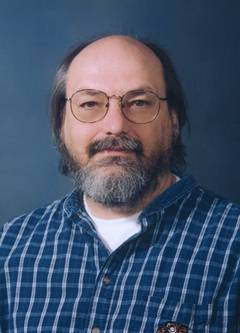
\includegraphics[width=.5\textwidth]{img/thompson02.jpg}
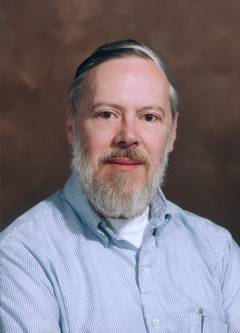
\includegraphics[width=.5\textwidth]{img/ritchie02.jpg}
\end{exampleblock}
\end{column}
\end{columns}
\end{frame}
\begin{frame}
\frametitle{出埃及记(1971-1983)}
\label{sec-2-1-2}
\begin{columns}
\begin{column}{0.6\textwidth}
%% Unix的发展演变
\label{sec-2-1-2-1}
\begin{itemize}

\item 1971年:C语言诞生
\label{sec-2-1-2-2}%

\item 1973年:Unix完全用C重写
\label{sec-2-1-2-3}%

\item 1975年:Unix V6版发布
\label{sec-2-1-2-4}%

\item 1977年:Bill Joy发布BSD v1版
\label{sec-2-1-2-5}%

\item 1983年:BSD 4.2上首次实现TCP/IP
\label{sec-2-1-2-6}%
\end{itemize} % ends low level
\end{column}
\begin{column}{0.4\textwidth}
\begin{exampleblock}{Unix history}
\label{sec-2-1-2-7}

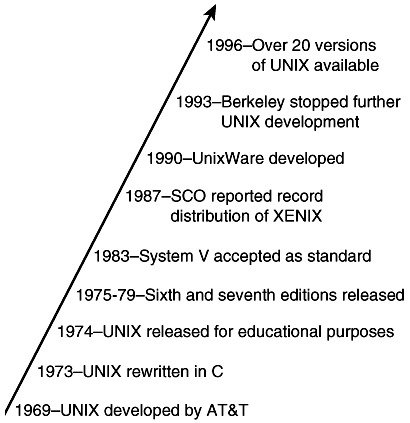
\includegraphics[width=1\textwidth]{img/unix-history.jpg}
\end{exampleblock}
\end{column}
\end{columns}
\end{frame}
\subsection{2.2 Linux诞生的基础}
\label{sec-2-2}
\begin{frame}
\frametitle{Minix系统}
\label{sec-2-2-1}
\begin{columns}
\begin{column}{0.6\textwidth}
%% minix
\label{sec-2-2-1-1}
\begin{itemize}

\item Unix商业化,源代码封闭
\label{sec-2-2-1-2}%

\item 荷兰教授Andrew S. Tanenbaum开发Minix
\label{sec-2-2-1-3}%

\item 类Unix、小巧、免费、教学
\label{sec-2-2-1-4}%
\end{itemize} % ends low level
\end{column}
\begin{column}{0.4\textwidth}
\begin{exampleblock}{Tanenbaum}
\label{sec-2-2-1-5}

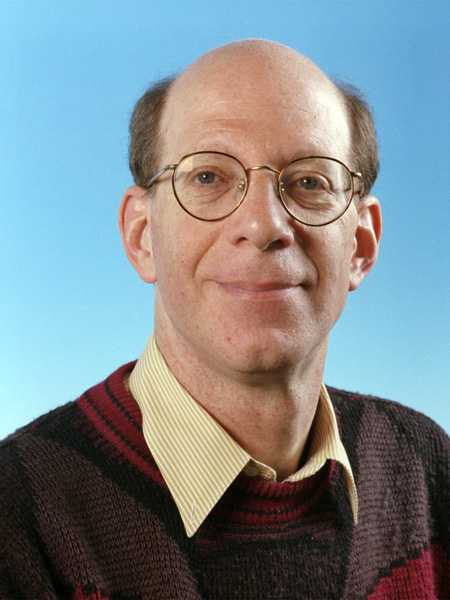
\includegraphics[width=1\textwidth]{img/ast.jpg}
\end{exampleblock}
\end{column}
\end{columns}
\end{frame}
\begin{frame}
\frametitle{Internet}
\label{sec-2-2-2}
\begin{itemize}

\item 80年代,Internet逐渐形成
\label{sec-2-2-2-1}%

\item 早期以技术用户为主
\label{sec-2-2-2-2}%

\item 通过网络切磋技术、协同工作、发布和获取软件代码
\label{sec-2-2-2-3}%

\item 形成植根于Internet的“黑客”文化
\label{sec-2-2-2-4}%
\end{itemize} % ends low level
\end{frame}
\begin{frame}
\frametitle{GNU}
\label{sec-2-2-3}
\begin{columns}
\begin{column}{0.5\textwidth}
%% 自由软件运动
\label{sec-2-2-3-1}
\begin{itemize}

\item 1983年,MIT的Richard Stallman开创GNU计划
\label{sec-2-2-3-2}%

\item GNU致力于开发一个自由的类Unix系统
\label{sec-2-2-3-3}%

\item 1988年,发布GPL许可协议用以保护自由软件
\label{sec-2-2-3-4}%

\item 1991年,GNU完成除内核外几乎所有必备软件的开发
\label{sec-2-2-3-5}%
\end{itemize} % ends low level
\end{column}
\begin{column}{0.5\textwidth}
\begin{exampleblock}{Richard Stallman and GNU}
\label{sec-2-2-3-6}

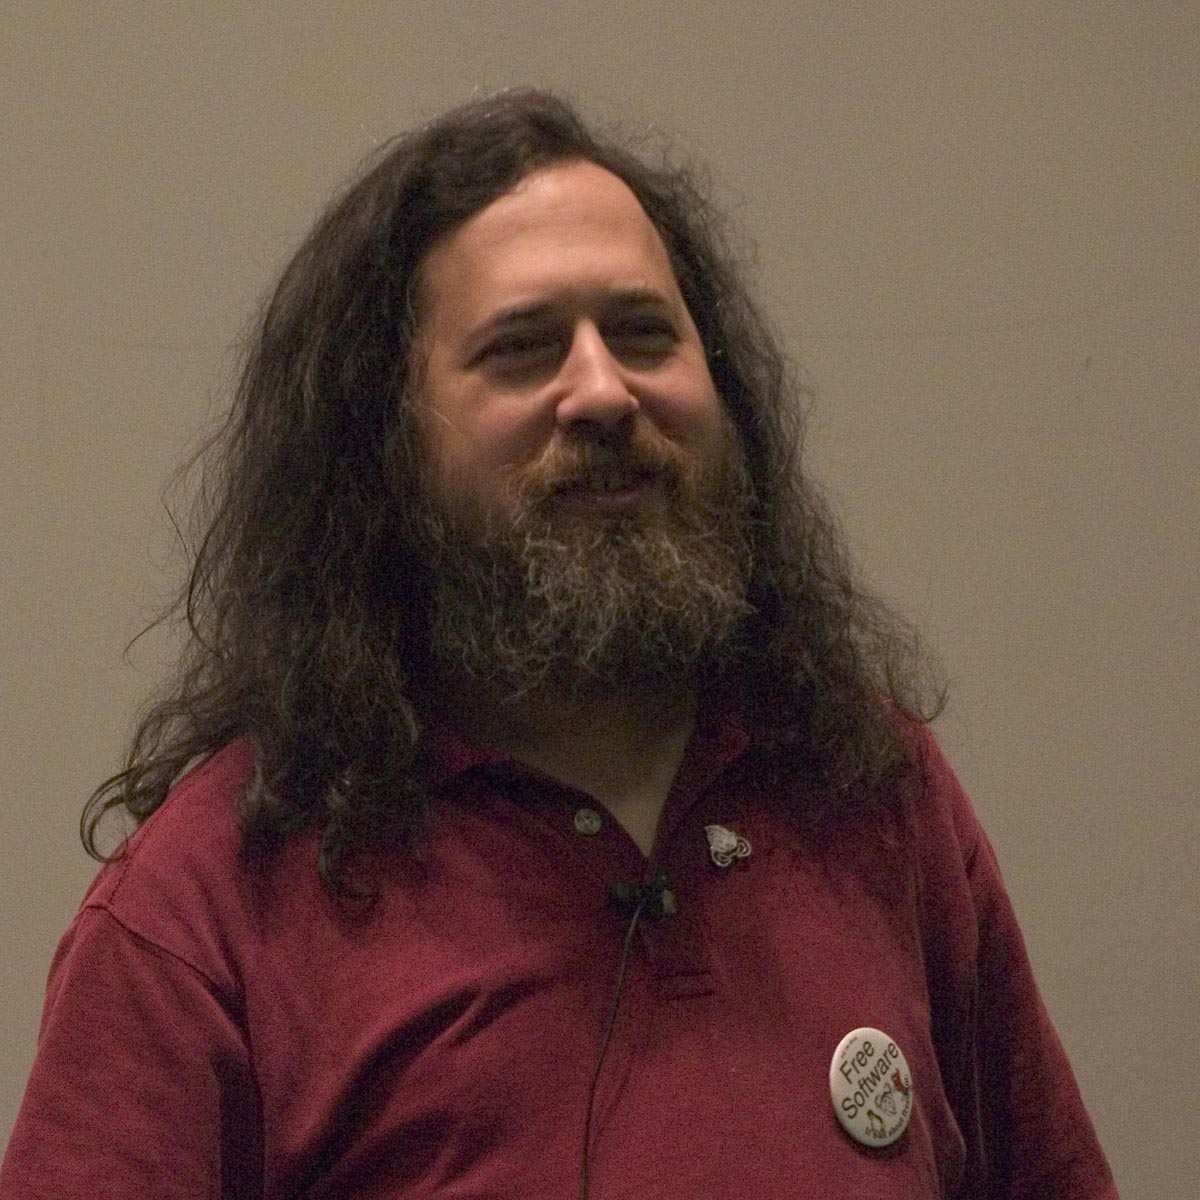
\includegraphics[width=.5\textwidth]{img/stallman.jpg}

\includegraphics[width=.5\textwidth]{img/gnu.jpg}
\end{exampleblock}
\end{column}
\end{columns}
\end{frame}
\begin{frame}
\frametitle{自由软件}
\label{sec-2-2-4}
\begin{itemize}

\item 自由软件赋予软件使用者四种自由:
\label{sec-2-2-4-1}%
\begin{itemize}

\item (freedom 0)为任何目的自由运行该软件的自由;
\label{sec-2-2-4-1-1}%

\item (freedom 1)有研究该软件如何运行,以及按需修改该软件的自由;
\label{sec-2-2-4-1-2}%

\item (freedom 2)有重新发布该软件拷贝的自由;
\label{sec-2-2-4-1-3}%

\item (freedom 3)有改进该软件,以及向公众发布改进的自由,这样整个社群都可受惠。
\label{sec-2-2-4-1-4}%
\end{itemize} % ends low level

\item 源代码开放是获得自由1和自由3的前提条件!
\label{sec-2-2-4-2}%
\end{itemize} % ends low level
\end{frame}
\begin{frame}
\frametitle{GPL}
\label{sec-2-2-5}
\begin{columns}
\begin{column}{0.6\textwidth}
%% GPL
\label{sec-2-2-5-1}
\begin{itemize}

\item 当开发者以GNU GPL作为软件许可证发布其软件时,该软件就成为自由软件并能保持自由软件的性质。
\label{sec-2-2-5-2}%

\item GPL规定的版权为Copyleft, 它允许任何人修改并重新分发自由软件,但要求保证该软件是仍然是自由软件。
\label{sec-2-2-5-3}%

\item Copyright(商业版权)是为了限制用户
\label{sec-2-2-5-4}%

\item Copyleft(自由版权)是为了维护用户自由的权力
\label{sec-2-2-5-5}%
\end{itemize} % ends low level
\end{column}
\begin{column}{0.4\textwidth}
\begin{exampleblock}{Left or Right?}
\label{sec-2-2-5-6}


\includegraphics[width=1\textwidth]{img/copy.jpg}
\end{exampleblock}
\end{column}
\end{columns}
\end{frame}
\subsection{2.3 Linux简介}
\label{sec-2-3}
\begin{frame}
\frametitle{Linux的诞生}
\label{sec-2-3-1}
\begin{columns}
\begin{column}{0.5\textwidth}
%% Linux诞生
\label{sec-2-3-1-1}
\begin{itemize}

\item 1991年8月25日,21岁的芬兰赫尔辛基大学计算机科学系二年级学生Linus Torvalds在comp.os.minix新闻组中宣告了Linux的诞生。
\label{sec-2-3-1-2}%
\end{itemize} % ends low level
\end{column}
\begin{column}{0.5\textwidth}
\begin{exampleblock}{Linux和Tux}
\label{sec-2-3-1-3}

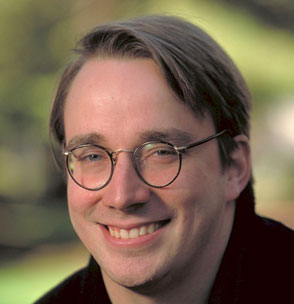
\includegraphics[width=.5\textwidth]{img/linus.jpg}

\includegraphics[width=.5\textwidth]{img/tux.jpg}
\end{exampleblock}
\end{column}
\end{columns}
\end{frame}
\begin{frame}
\frametitle{Linux的快速发展}
\label{sec-2-3-2}
\begin{columns}
\begin{column}{0.6\textwidth}
%% Linux的成功基础
\label{sec-2-3-2-1}
\begin{itemize}

\item Linux为什么会成功?
\label{sec-2-3-2-2}%
\begin{itemize}

\item 站在GNU的肩膀上
\label{sec-2-3-2-2-1}%

\item 采用GPL许可协议发布
\label{sec-2-3-2-2-2}%

\item 通过Internet协作开发
\label{sec-2-3-2-2-3}%
\end{itemize} % ends low level

\item 今天,Linux已经成长为业界最重要的操作系统,得到几乎所有业界大公司的支持,也是目前运行硬件平台最多的操作系统。
\label{sec-2-3-2-3}%
\end{itemize} % ends low level
\end{column}
\begin{column}{0.4\textwidth}
\begin{exampleblock}{GNU/Linux}
\label{sec-2-3-2-4}


\includegraphics[width=1\textwidth]{img/gnu-linux.jpg}
\end{exampleblock}
\end{column}
\end{columns}
\end{frame}
\begin{frame}
\frametitle{Linux的快速发展}
\label{sec-2-3-3}

\begin{center}
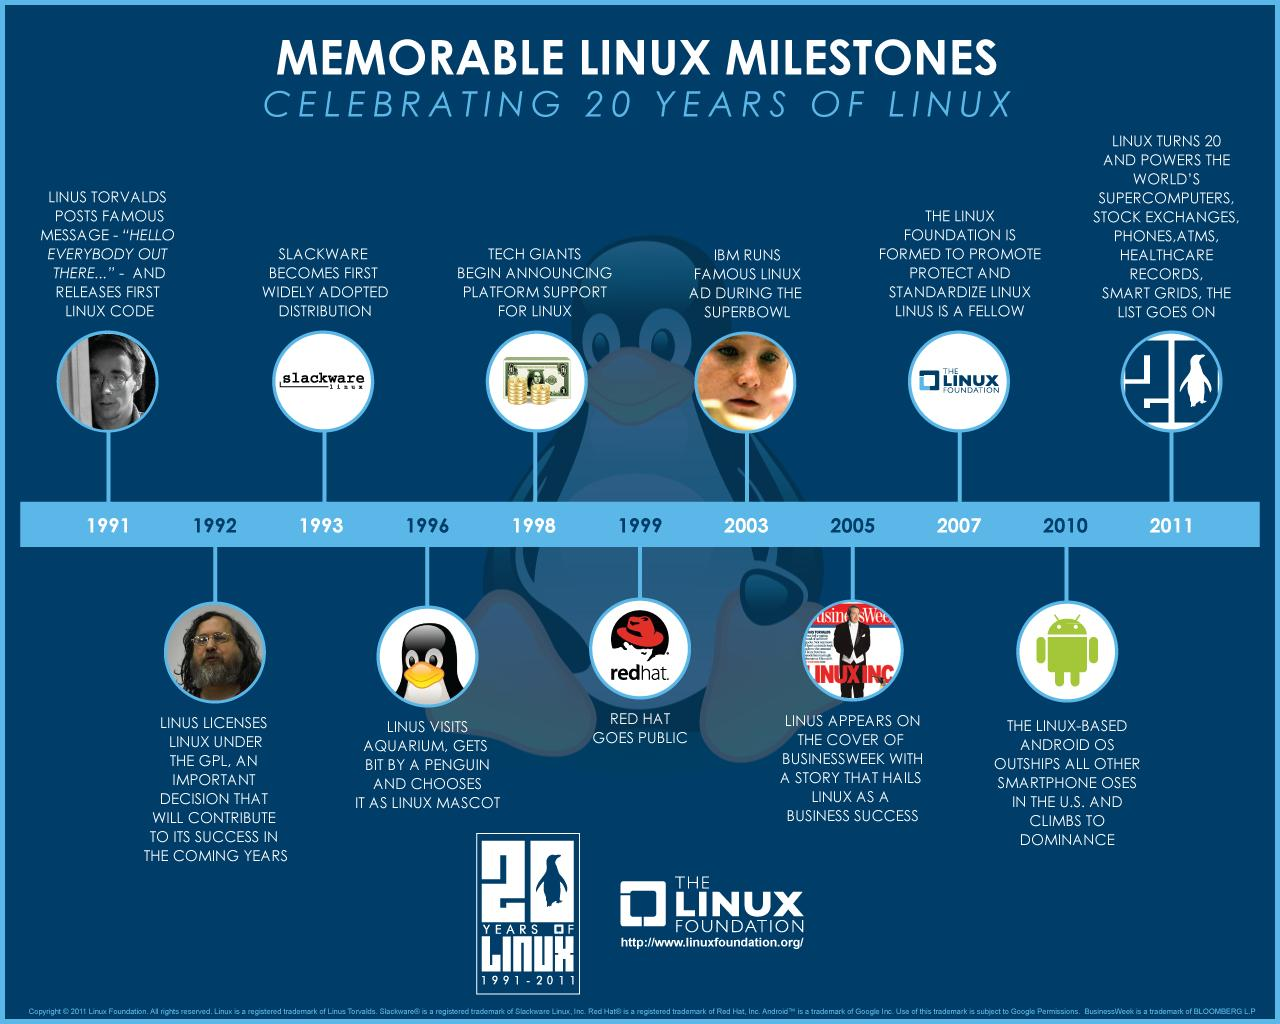
\includegraphics[width=.9\linewidth]{img/20year.jpg}
\end{center}
\end{frame}
\begin{frame}
\frametitle{Linux的特点}
\label{sec-2-3-4}
\begin{itemize}

\item 基于UNIX设计,性能出色
\label{sec-2-3-4-1}%

\item 遵照GPL许可,自由软件
\label{sec-2-3-4-2}%

\item 符合POSIX标准,兼容性好
\label{sec-2-3-4-3}%

\item 可移植性好
\label{sec-2-3-4-4}%

\item 网络功能强大
\label{sec-2-3-4-5}%

\item 安全性好
\label{sec-2-3-4-6}%
\end{itemize} % ends low level
\end{frame}
\begin{frame}[fragile]
\frametitle{Linux的内核版本}
\label{sec-2-3-5}
\begin{itemize}

\item Linux版本号由3个数字组成:r.x.y
\label{sec-2-3-5-1}%
\begin{itemize}

\item r:目前发布的Kernel主版本
\label{sec-2-3-5-1-1}%

\item x:偶数是稳定版本,奇数是开发版本
\label{sec-2-3-5-1-2}%

\item y:错误修补次数
\label{sec-2-3-5-1-3}%
\end{itemize} % ends low level

\item 查看系统的内核版本号\\
\label{sec-2-3-5-2}%
\begin{minted}[]{bash}
uname -r
\end{minted}

\item 内核官网
\label{sec-2-3-5-3}%
\begin{itemize}

\item \href{https://www.kernel.org}{www.kernel.org}
\label{sec-2-3-5-3-1}%
\end{itemize} % ends low level
\end{itemize} % ends low level
\end{frame}
\begin{frame}
\frametitle{Linux发行版}
\label{sec-2-3-6}
\begin{itemize}

\item 各IT厂商和组织把Linux内核与大量应用软件按各自的方式打包成便于安装的形式,就称为Linux发行版
\label{sec-2-3-6-1}%

\item 发行版本号随发布者的不同而不同,与系统内核版本号相对独立
\label{sec-2-3-6-2}%

\item 目前世界上已经有超过百种不同的Linux发行版
\label{sec-2-3-6-3}%
\begin{itemize}

\item \href{http://distrowatch.com}{http://distrowatch.com}
\label{sec-2-3-6-3-1}%
\end{itemize} % ends low level
\end{itemize} % ends low level
\end{frame}
\begin{frame}
\frametitle{Linux发行版}
\label{sec-2-3-7}

\begin{center}

\includegraphics[width=.9\linewidth]{img/distri.jpg}
\end{center}
\end{frame}
\subsection{2.4 Linux vs. Windows}
\label{sec-2-4}
\begin{frame}
\frametitle{Windows和Linux}
\label{sec-2-4-1}
\begin{itemize}

\item Windows和Linux各有特点
\label{sec-2-4-1-1}%
\begin{itemize}

\item Windows是商业软件,Linux是自由软件
\label{sec-2-4-1-1-1}%

\item Windows图形界面友好,Linux命令行灵活高效
\label{sec-2-4-1-1-2}%

\item Windows易用性好,Linux定制性强
\label{sec-2-4-1-1-3}%

\item Windows像傻瓜相机,Linux像单反相机
\label{sec-2-4-1-1-4}%
\end{itemize} % ends low level

\item 在学习Linux时注意和Windows进行对比
\label{sec-2-4-1-2}%
\end{itemize} % ends low level
\end{frame}
\begin{frame}
\frametitle{无处不在的Linux}
\label{sec-2-4-2}
\begin{itemize}

\item Android基于Linux,每天有超过550,000部Android设备被激活。
\label{sec-2-4-2-1}%
\begin{center}
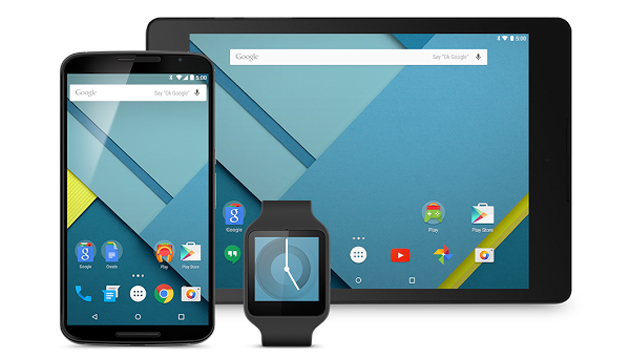
\includegraphics[width=.9\linewidth]{img/android.jpg}
\end{center}

\end{itemize} % ends low level
\end{frame}
\begin{frame}
\frametitle{无处不在的Linux}
\label{sec-2-4-3}
\begin{itemize}

\item 当前全球top 500超级计算机中有469台运行Linux。
\label{sec-2-4-3-1}%
\begin{center}
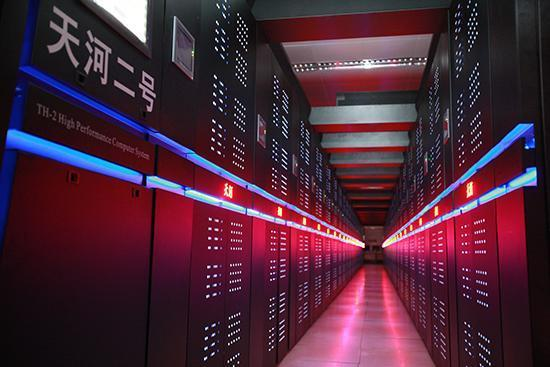
\includegraphics[width=.9\linewidth]{img/tianhe.jpg}
\end{center}

\end{itemize} % ends low level
\end{frame}
\begin{frame}
\frametitle{无处不在的Linux}
\label{sec-2-4-4}
\begin{itemize}

\item 高铁运行管理
\label{sec-2-4-4-1}%
\begin{center}
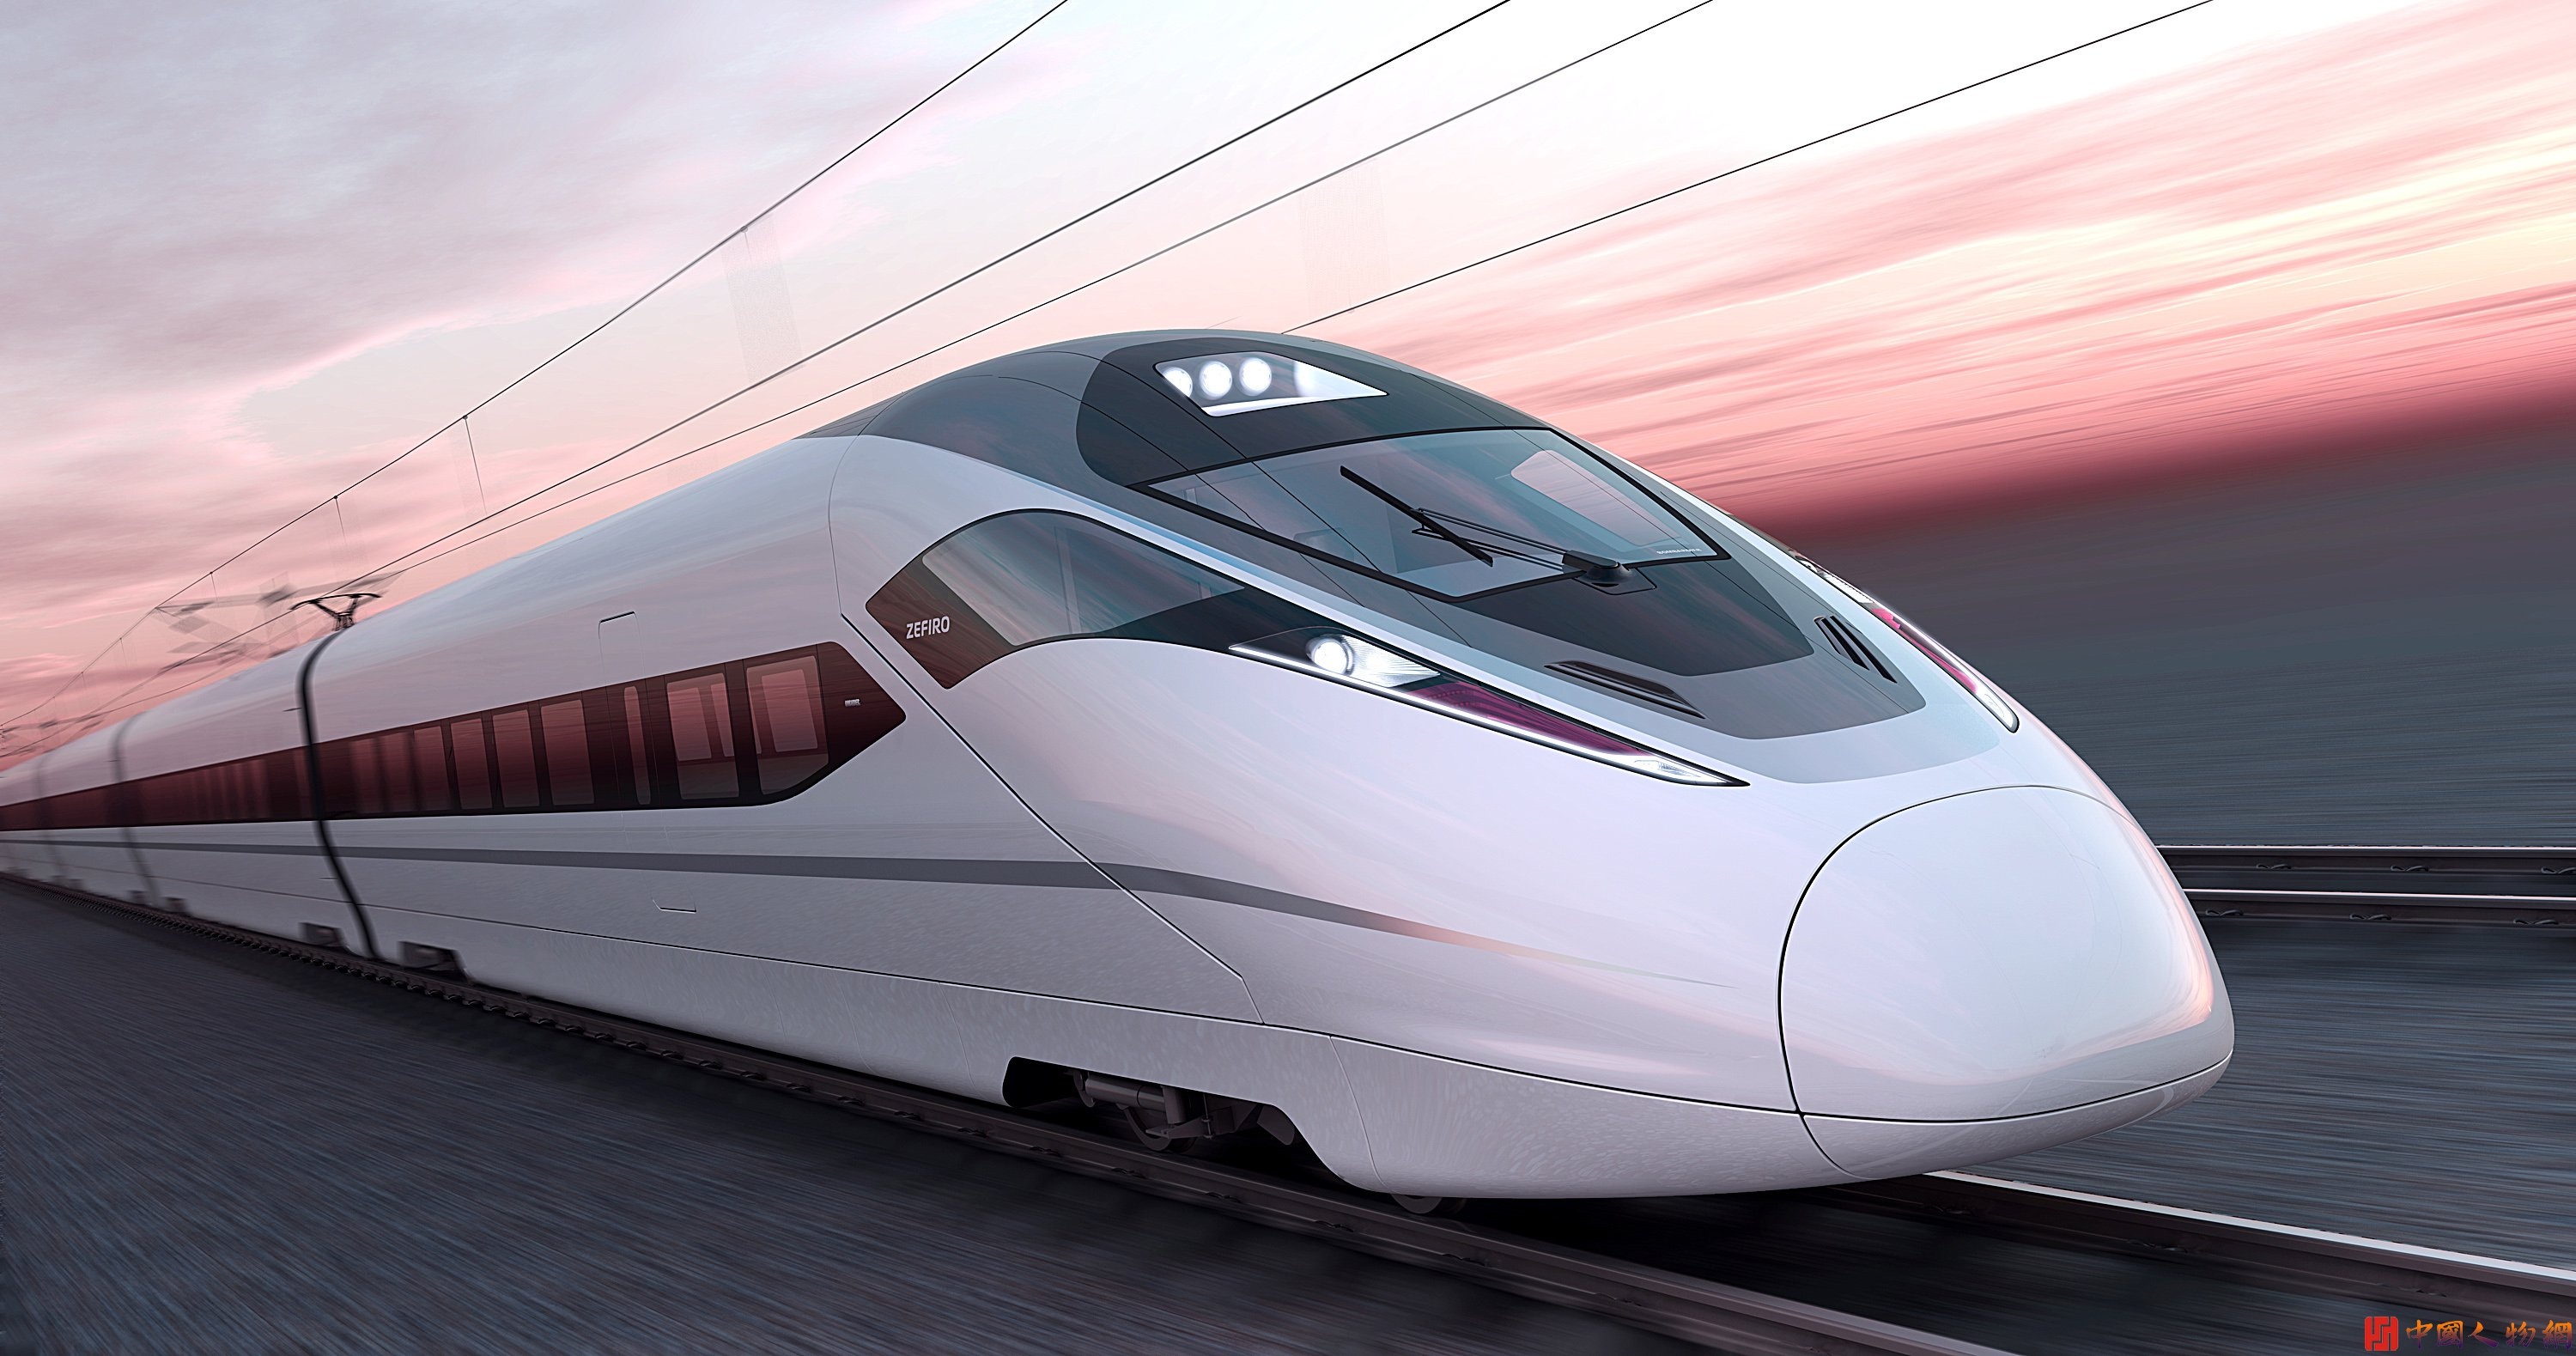
\includegraphics[width=.9\linewidth]{img/train.jpg}
\end{center}

\end{itemize} % ends low level
\end{frame}
\begin{frame}
\frametitle{无处不在的Linux}
\label{sec-2-4-5}
\begin{itemize}

\item 交通控制系统
\label{sec-2-4-5-1}%
\begin{center}
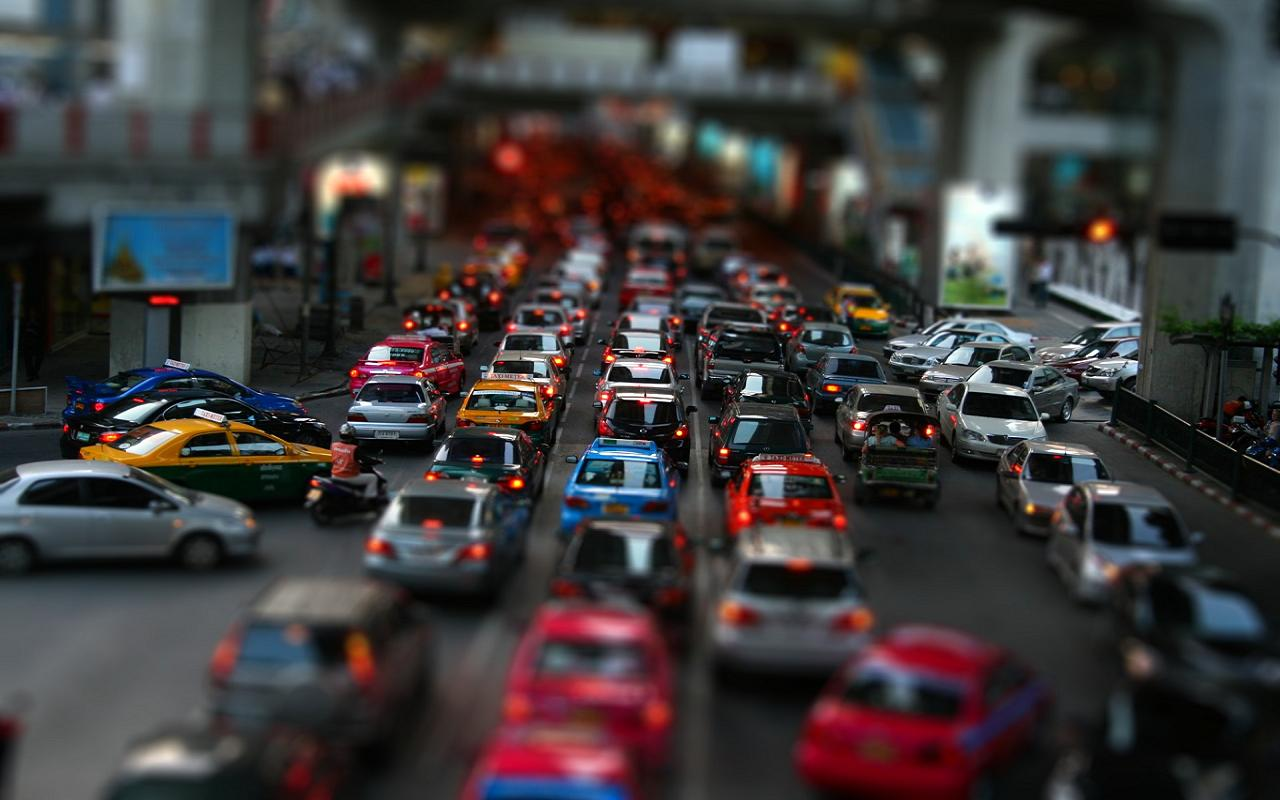
\includegraphics[width=.9\linewidth]{img/traffic2.jpg}
\end{center}

\end{itemize} % ends low level
\end{frame}
\begin{frame}
\frametitle{无处不在的Linux}
\label{sec-2-4-6}
\begin{itemize}

\item 工业制造
\label{sec-2-4-6-1}%
\begin{center}
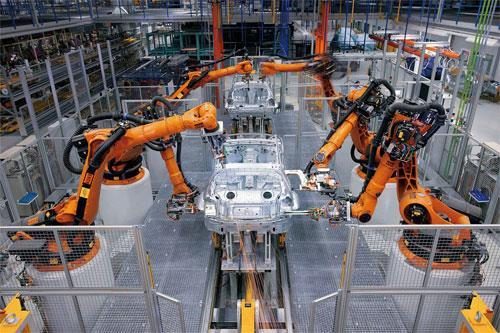
\includegraphics[width=.9\linewidth]{img/industry.jpg}
\end{center}

\end{itemize} % ends low level
\end{frame}
\begin{frame}
\frametitle{无处不在的Linux}
\label{sec-2-4-7}
\begin{itemize}

\item 智能农牧业
\label{sec-2-4-7-1}%
\begin{center}
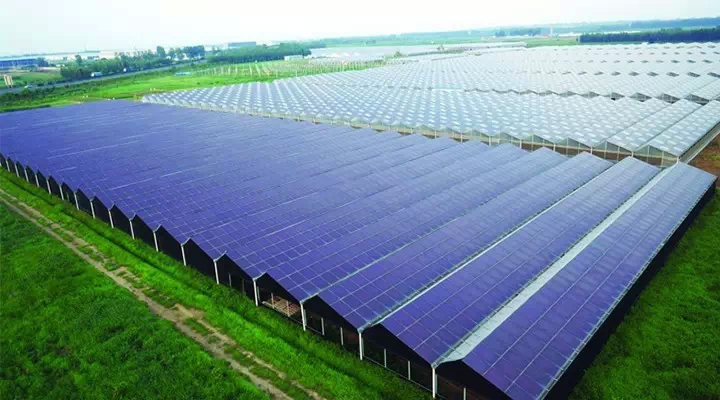
\includegraphics[width=.9\linewidth]{img/nongye.jpg}
\end{center}

\end{itemize} % ends low level
\end{frame}
\begin{frame}
\frametitle{无处不在的Linux}
\label{sec-2-4-8}
\begin{itemize}

\item 金融证券
\label{sec-2-4-8-1}%
\begin{center}
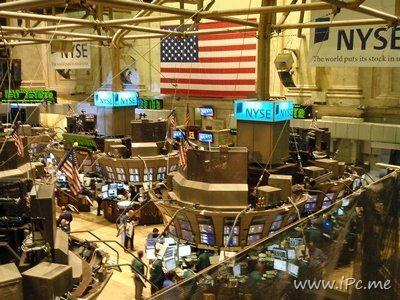
\includegraphics[width=.9\linewidth]{img/jinrong.jpg}
\end{center}

\end{itemize} % ends low level
\end{frame}
\begin{frame}
\frametitle{无处不在的Linux}
\label{sec-2-4-9}
\begin{itemize}

\item 高能粒子加速器
\label{sec-2-4-9-1}%
\begin{center}
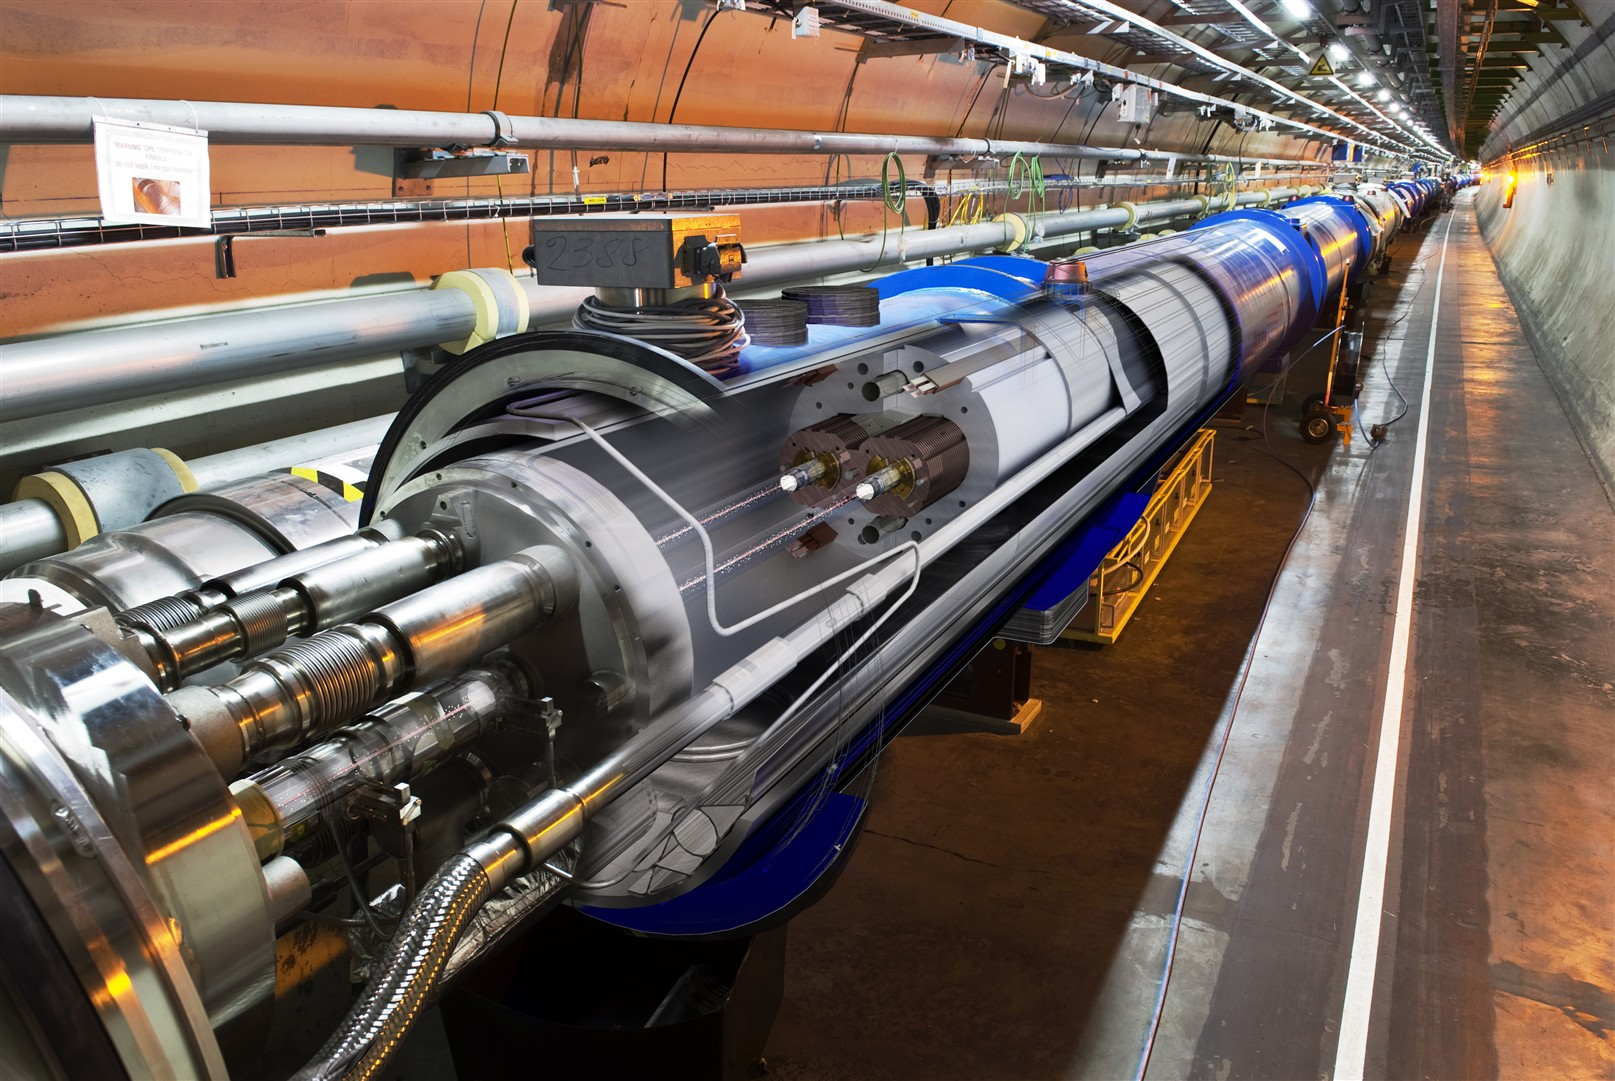
\includegraphics[width=.9\linewidth]{img/jiasuqi.jpg}
\end{center}

\end{itemize} % ends low level
\end{frame}
\begin{frame}
\frametitle{无处不在的Linux}
\label{sec-2-4-10}
\begin{itemize}

\item 核潜艇
\label{sec-2-4-10-1}%
\begin{center}
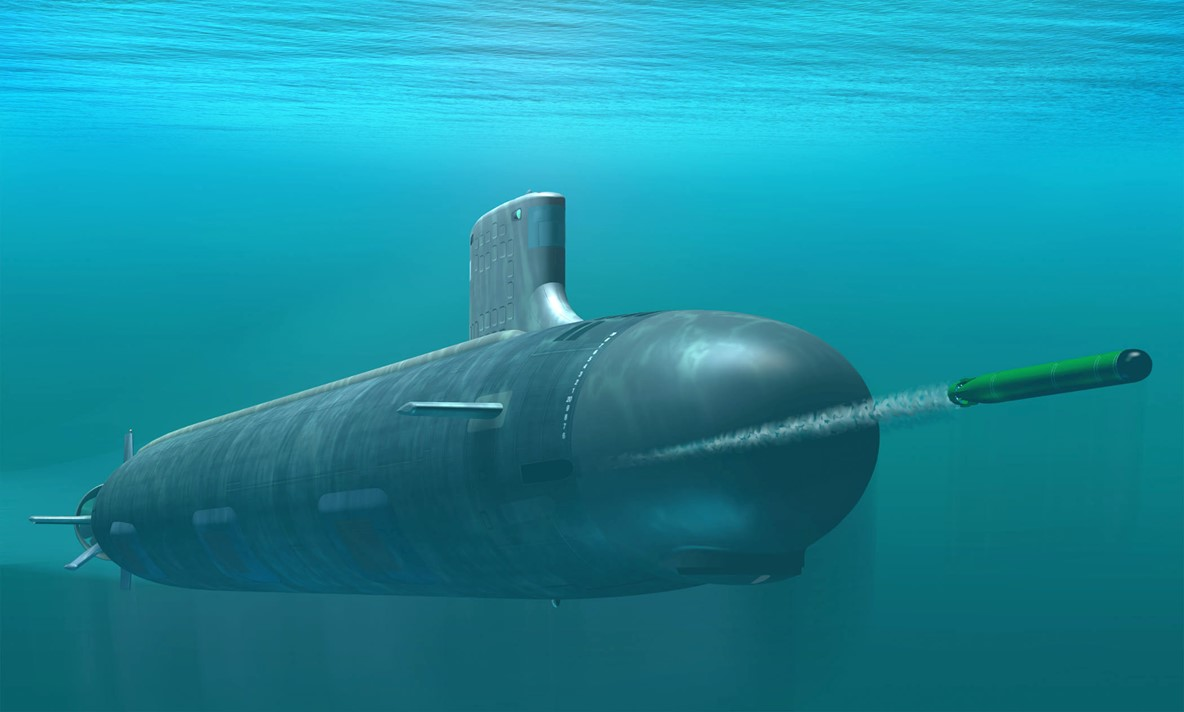
\includegraphics[width=.9\linewidth]{img/nuclear.jpg}
\end{center}

\end{itemize} % ends low level
\end{frame}
\begin{frame}
\frametitle{无处不在的Linux}
\label{sec-2-4-11}
\begin{itemize}

\item 影视娱乐
\label{sec-2-4-11-1}%
\begin{center}

\includegraphics[width=.9\linewidth]{img/jingang.jpg}
\end{center}

\end{itemize} % ends low level
\end{frame}
\begin{frame}
\frametitle{You are here}
\label{sec-2-4-12}

\begin{center}
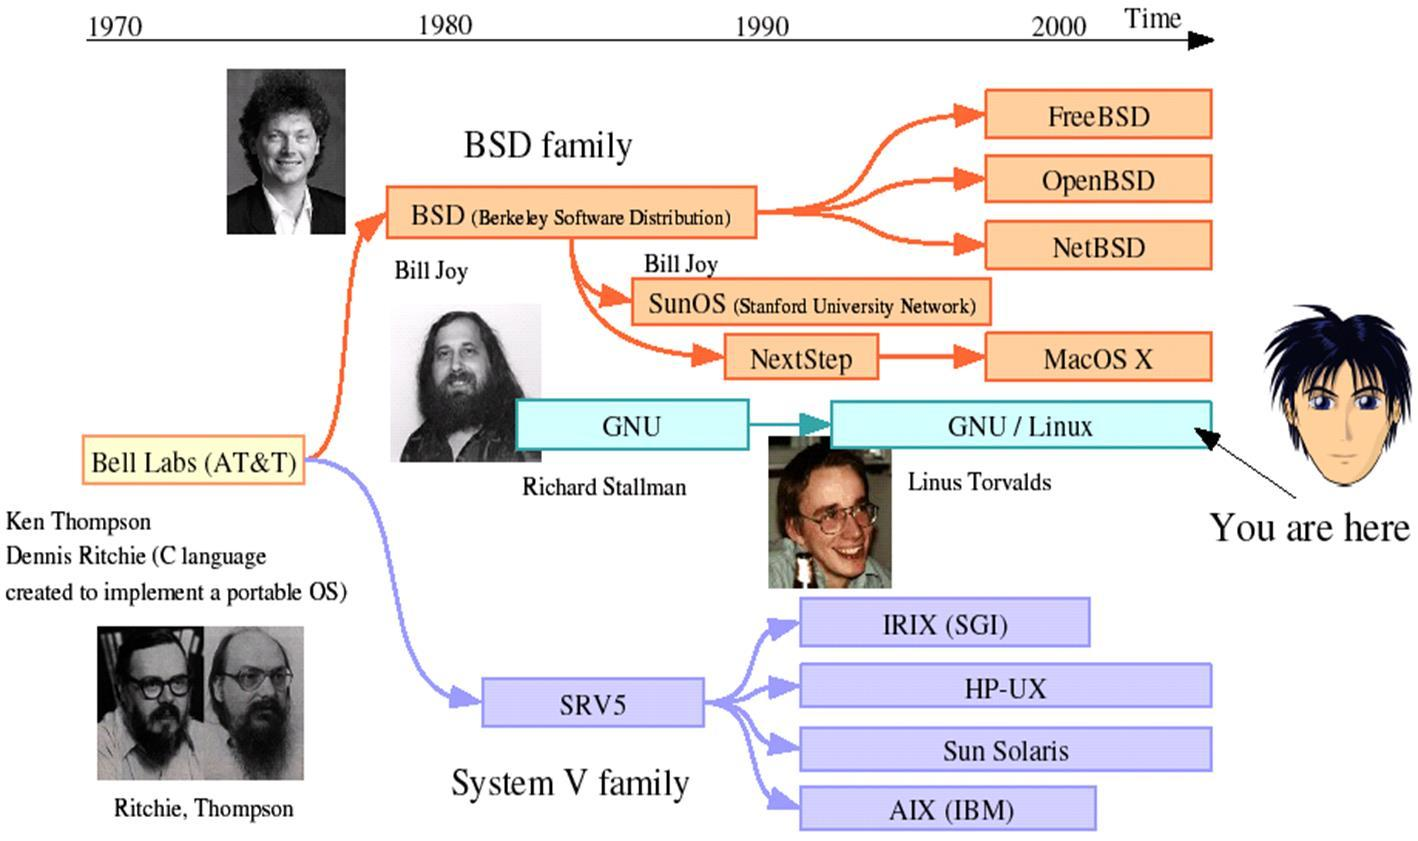
\includegraphics[width=.9\linewidth]{img/here.jpg}
\end{center}
\end{frame}
\section{Linux安装}
\label{sec-3}
\subsection{3.1 通过虚拟机安装Linux}
\label{sec-3-1}
\begin{frame}
\frametitle{虚拟机软件}
\label{sec-3-1-1}
\begin{itemize}

\item 常用虚拟机软件
\label{sec-3-1-1-1}%
\begin{itemize}

\item vmware
\label{sec-3-1-1-1-1}%

\item virtualbox
\label{sec-3-1-1-1-2}%

\item kvm
\label{sec-3-1-1-1-3}%
\end{itemize} % ends low level

\item 利用虚拟机软件安装操作系统
\label{sec-3-1-1-2}%
\begin{enumerate}
\item 创建虚拟机(指定虚拟机硬件参数)
\item 为虚拟机挂载操作系统安装光盘
\item 在虚拟机上安装操作系统
\end{enumerate}
\end{itemize} % ends low level
\end{frame}
\subsection{3.2 Linux分区}
\label{sec-3-2}
\begin{frame}
\frametitle{分区与目录}
\label{sec-3-2-1}
\begin{itemize}

\item 硬盘分区规则
\label{sec-3-2-1-1}%
\begin{itemize}

\item 一块普通硬盘最少要分1个主分区,最多能分4个主分区
\label{sec-3-2-1-1-1}%

\item 也可以分1-3个主分区,外加一个扩展分区
\label{sec-3-2-1-1-2}%

\item 扩展分区内可以划分更多的逻辑分区
\label{sec-3-2-1-1-3}%
\end{itemize} % ends low level

\item Windos分区与Linux分区
\label{sec-3-2-1-2}%
\begin{itemize}

\item Windows
\label{sec-3-2-1-2-1}%
\begin{itemize}

\item 多根目录:每个分区都有一个根目录
\label{sec-3-2-1-2-1-1}%
\end{itemize} % ends low level

\item Linux
\label{sec-3-2-1-2-2}%
\begin{itemize}

\item 单根目录:整个系统只有一个根目录
\label{sec-3-2-1-2-2-1}%

\item 所有分区都挂载在目录树上的某个目录(称为挂载点)下面
\label{sec-3-2-1-2-2-2}%

\item 根分区挂载于/目录,其他分区挂载于根目录下的子目录
\label{sec-3-2-1-2-2-3}%

\item 对分区的文件访问,通过相应的挂载点进行
\label{sec-3-2-1-2-2-4}%
\end{itemize} % ends low level
\end{itemize} % ends low level
\end{itemize} % ends low level
\end{frame}
\begin{frame}
\frametitle{Linux目录结构}
\label{sec-3-2-2}

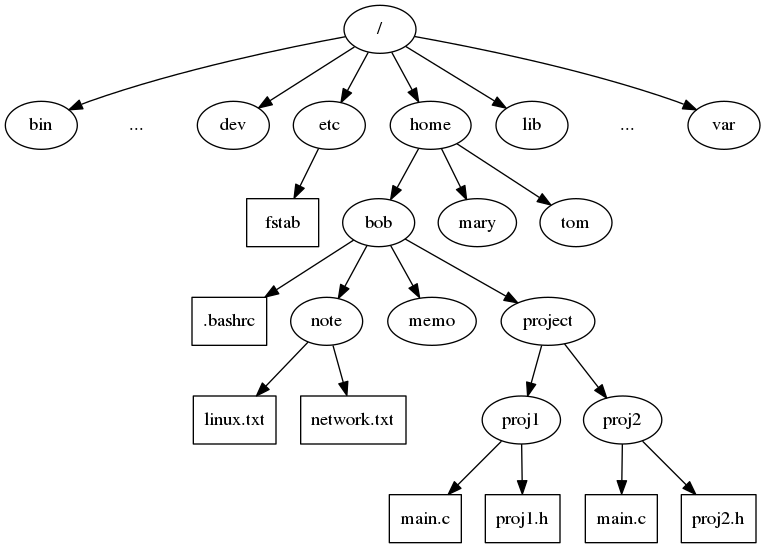
\includegraphics[width=.9\linewidth]{img/dirtree.pdf}
\end{frame}
\begin{frame}
\frametitle{分区方案}
\label{sec-3-2-3}
\begin{itemize}

\item /分区+Swap交换分区
\label{sec-3-2-3-1}%
\begin{itemize}

\item swap分区:物理内存不够时进行内存交换,无挂载点
\label{sec-3-2-3-1-1}%

\item 一般设为物理内存的1-2倍大小
\label{sec-3-2-3-1-2}%
\end{itemize} % ends low level

\item /分区+/boot分区+Swap交换分区
\label{sec-3-2-3-2}%
\begin{itemize}

\item /boot 用于存放系统引导程序、系统内核等
\label{sec-3-2-3-2-1}%

\item 一般不超过500MB
\label{sec-3-2-3-2-2}%
\end{itemize} % ends low level

\item 其他常用来挂载分区的目录
\label{sec-3-2-3-3}%
\begin{itemize}

\item /home 用于存放用户个人的数据
\label{sec-3-2-3-3-1}%

\item /usr 用于存放不太变化的内容,如应用程序和文档
\label{sec-3-2-3-3-2}%

\item /tmp 用于存放临时文件
\label{sec-3-2-3-3-3}%

\item /var 用于存放经常变化的内容,如日志、邮件等
\label{sec-3-2-3-3-4}%

\item /opt 用于存放系统附加软件包
\label{sec-3-2-3-3-5}%
\end{itemize} % ends low level
\end{itemize} % ends low level
\end{frame}
\begin{frame}
\frametitle{分区名称}
\label{sec-3-2-4}
\begin{itemize}

\item IDE接口设备及其分区
\label{sec-3-2-4-1}%
\begin{itemize}

\item 硬盘:/dev/hda /dev/hdb \ldots{}
\label{sec-3-2-4-1-1}%

\item 分区:/dev/hda1 /dev/hda2 \ldots{}
\label{sec-3-2-4-1-2}%
\end{itemize} % ends low level

\item SCSI接口设备及其分区
\label{sec-3-2-4-2}%
\begin{itemize}

\item 硬盘:/dev/sda /dev/sdb \ldots{}
\label{sec-3-2-4-2-1}%

\item 分区:/dev/sdb1 /dev/sdb3 \ldots{}
\label{sec-3-2-4-2-2}%
\end{itemize} % ends low level

\item 注意
\label{sec-3-2-4-3}%
\begin{itemize}

\item 逻辑分区的编号从5开始
\label{sec-3-2-4-3-1}%

\item SATA接口和USB接口也被认作SCSI接口
\label{sec-3-2-4-3-2}%
\end{itemize} % ends low level

\item 设备文件名 vs. 挂载点
\label{sec-3-2-4-4}%
\begin{itemize}

\item 设备文件名:是一个文件,代表设备本身
\label{sec-3-2-4-4-1}%

\item 挂载点:是一个目录,可用于访问设备内容
\label{sec-3-2-4-4-2}%

\item 例:将/dev/cdrom挂载到/media/cdrom
\label{sec-3-2-4-4-3}%
\end{itemize} % ends low level
\end{itemize} % ends low level
\end{frame}
\subsection{3.3 虚拟机网络设置}
\label{sec-3-3}
\begin{frame}
\frametitle{NAT}
\label{sec-3-3-1}
\begin{itemize}

\item 虚拟机通过虚拟NAT设备连接到主机,并可通过主机连接外部网络
\label{sec-3-3-1-1}%
\begin{center}
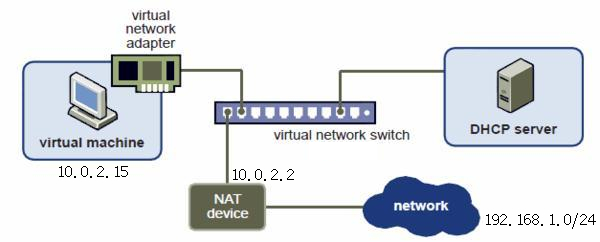
\includegraphics[width=.9\linewidth]{img/nat.jpg}
\end{center}

\end{itemize} % ends low level
\end{frame}
\begin{frame}
\frametitle{Bridged}
\label{sec-3-3-2}
\begin{itemize}

\item 虚拟机通过虚拟交换机连接到主机所在局域网
\label{sec-3-3-2-1}%
\begin{center}
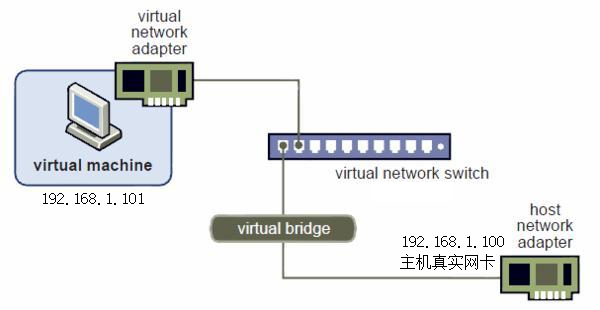
\includegraphics[width=.9\linewidth]{img/bridged.jpg}
\end{center}

\end{itemize} % ends low level
\end{frame}
\begin{frame}
\frametitle{Host-only}
\label{sec-3-3-3}
\begin{itemize}

\item 虚拟机通过虚拟交换机连接到主机虚拟网卡所连的局域网
\label{sec-3-3-3-1}%
\begin{center}
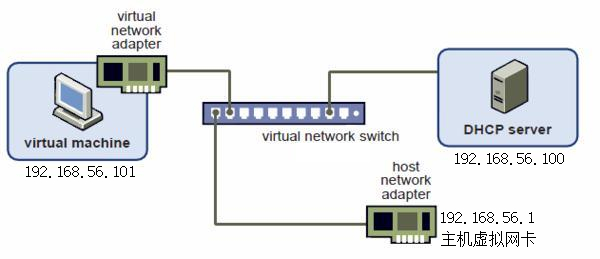
\includegraphics[width=.9\linewidth]{img/host-only.jpg}
\end{center}

\end{itemize} % ends low level
\end{frame}
\begin{frame}
\frametitle{Internel}
\label{sec-3-3-4}
\begin{itemize}

\item 虚拟机通过虚拟交换机连接到虚拟机内部的虚拟局域网
\label{sec-3-3-4-1}%
\begin{center}
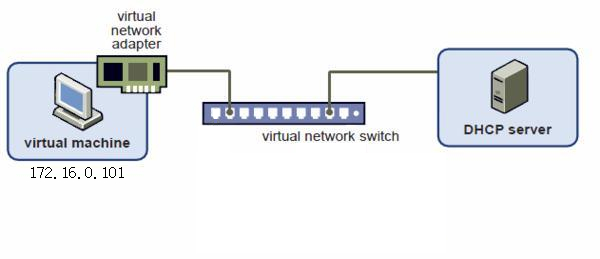
\includegraphics[width=.9\linewidth]{img/internal.jpg}
\end{center}

\end{itemize} % ends low level
\end{frame}
\subsection{3.4 通过ssh远程登录Linux}
\label{sec-3-4}
\begin{frame}[fragile]
\frametitle{ssh客户端}
\label{sec-3-4-1}
\begin{itemize}

\item Linux客户端\\
\label{sec-3-4-1-1}%
\begin{minted}[]{bash}
ssh -l username 192.168.56.102
ssh username@192.168.56.102
ssh -p 22 -l username 192.168.56.102
\end{minted}

\item Windows客户端
\label{sec-3-4-1-2}%
\begin{itemize}

\item putty
\label{sec-3-4-1-2-1}%

\item SecureCRT
\label{sec-3-4-1-2-2}%
\end{itemize} % ends low level

\item 主机访问NAT后的虚拟机
\label{sec-3-4-1-3}%
\begin{itemize}

\item 虚拟机上设置端口转发:假设设置127.0.0.1:2222-->10.0.2.15:22\\
\label{sec-3-4-1-3-1}%
\begin{minted}[]{bash}
ssh -p 2222 -l username 127.0.0.1
\end{minted}
\end{itemize} % ends low level
\end{itemize} % ends low level
\end{frame}
\subsection{3.5 虚拟机管理}
\label{sec-3-5}
\begin{frame}
\frametitle{虚拟机常用操作}
\label{sec-3-5-1}
\begin{itemize}

\item 快照备份与恢复
\label{sec-3-5-1-1}%
\begin{itemize}

\item 可备份某一时刻的系统状态,将来虚拟机由于误操作出现问题时可以恢复到备份时的状态。
\label{sec-3-5-1-1-1}%

\item 可以对虚拟机状态进行多次备份,并随时切换到某个备份状态。
\label{sec-3-5-1-1-2}%
\end{itemize} % ends low level

\item 利用虚拟硬盘快速创建虚拟机
\label{sec-3-5-1-2}%
\begin{itemize}

\item 利用已经安装好了虚拟机的虚拟硬盘快速创建新的虚拟机。
\label{sec-3-5-1-2-1}%
\end{itemize} % ends low level

\item 虚拟机复制
\label{sec-3-5-1-3}%
\begin{itemize}

\item 利用现有虚拟机快速克隆出新的虚拟机。
\label{sec-3-5-1-3-1}%
\end{itemize} % ends low level
\end{itemize} % ends low level
\end{frame}
\section{Linux入门}
\label{sec-4}
\subsection{4.1 终端与多用户}
\label{sec-4-1}
\begin{frame}
\frametitle{终端与控制台}
\label{sec-4-1-1}
\begin{itemize}

\item 终端和控制台都不是个人电脑的概念,而是多人共用的小型中型大型计算机上的概念。
\label{sec-4-1-1-1}%
\begin{itemize}

\item 终端
\label{sec-4-1-1-1-1}%
\begin{itemize}

\item 字符终端
\label{sec-4-1-1-1-1-1}%

\item 图形终端
\label{sec-4-1-1-1-1-2}%
\end{itemize} % ends low level

\item 控制台
\label{sec-4-1-1-1-2}%
\begin{itemize}

\item 通过显示器和键盘接口与主机相连的键盘和显示器
\label{sec-4-1-1-1-2-1}%

\item 个人计算机只有控制台,没有终端
\label{sec-4-1-1-1-2-2}%
\end{itemize} % ends low level

\item 本地虚拟终端:在控制台上用软件虚拟出来的终端
\label{sec-4-1-1-1-3}%
\begin{itemize}

\item 图形终端:Ctrl-Alt-F1
\label{sec-4-1-1-1-3-1}%

\item 字符终端:Ctrl-Alt-F2\~{}Ctrl-Alt-F6
\label{sec-4-1-1-1-3-2}%
\begin{itemize}

\item 在字符终端上切换时,可以不按Ctrl键
\label{sec-4-1-1-1-3-2-1}%

\item 图形终端里面也有自己的虚拟字符终端
\label{sec-4-1-1-1-3-2-2}%
\end{itemize} % ends low level
\end{itemize} % ends low level

\item 远程虚拟终端
\label{sec-4-1-1-1-4}%
\begin{itemize}

\item 通过网络连接到计算机的虚拟终端。
\label{sec-4-1-1-1-4-1}%
\end{itemize} % ends low level
\end{itemize} % ends low level
\end{itemize} % ends low level
\end{frame}
\begin{frame}[fragile]
\frametitle{终端与多用户}
\label{sec-4-1-2}
\begin{itemize}

\item 多个终端可以供不同用户同时登录使用系统
\label{sec-4-1-2-1}%

\item 单个用户可以同时使用多个终端
\label{sec-4-1-2-2}%
\begin{itemize}

\item 用户可同时打开多个终端,每个终端上做不同的事情。
\label{sec-4-1-2-2-1}%
\end{itemize} % ends low level

\item 用户在终端登录后还可以切换为其他用户身份
\label{sec-4-1-2-3}%
\begin{itemize}

\item 系统管理员root可以随时切换为其他用户身份
\label{sec-4-1-2-3-1}%

\item 普通用户tom在知道其他用户的登录名和登录密码时,也可以切换为其他用户身份\\
\label{sec-4-1-2-3-2}%
\begin{verbatim}
# su - mary # root切换为mary
$ su - root # tom切换为root,会提示输入root密码
$ su -      # 同上
$ exit      # 返回原先用户身份,快捷键为Ctrl-d
\end{verbatim}
\end{itemize} % ends low level
\end{itemize} % ends low level
\end{frame}
\subsection{4.2 入门使用}
\label{sec-4-2}
\begin{frame}[fragile]
\frametitle{登录和注销}
\label{sec-4-2-1}
\begin{itemize}

\item 登录
\label{sec-4-2-1-1}%
\begin{itemize}

\item 系统提示login:
\label{sec-4-2-1-1-1}%

\item 输入用户名
\label{sec-4-2-1-1-2}%

\item 输入用户密码
\label{sec-4-2-1-1-3}%
\begin{itemize}

\item 注意:字符终端下输入密码时,系统会关闭屏幕回显。
\label{sec-4-2-1-1-3-1}%
\end{itemize} % ends low level
\end{itemize} % ends low level

\item 注销
\label{sec-4-2-1-2}%
\begin{itemize}

\item 注销代表用户离开,不等于关机
\label{sec-4-2-1-2-1}%

\item 注销命令\\
\label{sec-4-2-1-2-2}%
\begin{verbatim}
exit         # 快捷键为Ctrl-d
logout
\end{verbatim}
\end{itemize} % ends low level
\end{itemize} % ends low level
\end{frame}
\begin{frame}[fragile]
\frametitle{打个招呼吧}
\label{sec-4-2-2}
\begin{itemize}

\item echo\\
\label{sec-4-2-2-1}%
\begin{minted}[]{bash}
echo hello
echo nice to meet you!
echo "nice to meet you!"
echo 'nice to meet you!'
echo nice to meet you\!
echo "nice to meet you\!"
echo 'nice to meet you\!'
\end{minted}
\end{itemize} % ends low level
\begin{block}{试一试}
\label{sec-4-2-2-2}

请打印字符串It's time to learn linux!
\end{block}
\note{答案

echo It\'s time to learn linux!
echo ``It's time to learn linux''!
echo `It'\'' time to learn linux!'
}
\end{frame}
\begin{frame}[fragile]
\frametitle{打个招呼吧}
\label{sec-4-2-3}
\begin{itemize}

\item echo\\
\label{sec-4-2-3-1}%
\begin{minted}[]{bash}
echo hello \
nice to meet you!
echo 'hello
nice to meet you!'
echo "hello
nice to meet you."
echo -e 'hello\nnice to meet you!'
echo -e hello\nnice to meet you!
\end{minted}
\end{itemize} % ends low level
\begin{block}{试一试}
\label{sec-4-2-3-2}

请打印所有天干(甲乙丙丁戊己庚辛壬癸)地支(子丑寅卯辰巳午未申酉戌亥)的组合
\end{block}
\note{答案

echo \{甲,乙,丙,丁,戊,己,庚,辛,壬,癸\}{子,丑,寅,卯,辰,巳,午,未, 酉,戌,亥\}
}
\end{frame}
\begin{frame}[fragile]
\frametitle{看个时间}
\label{sec-4-2-4}
\begin{itemize}

\item 时间\\
\label{sec-4-2-4-1}%
\begin{minted}[]{bash}
date           #现在什么时间?
date +%H:%M    #现在几点几分?
date "+%B %d"  #今天几月几号?
date +%s       #打印纪元时(秒)

date --date "Oct 1 2016" +%A      #国庆节星期几呀?
date -s "2016-03-10 10:01:23"     #把时间调一下吧!
\end{minted}
\end{itemize} % ends low level
\note{备忘

echo `date +\%s`/265/24/3600 | bc  \#现在是纪元多少年呀?
clock -w                          \#把系统时间写入CMOS
}
\end{frame}
\begin{frame}[fragile]
\frametitle{查查日历}
\label{sec-4-2-5}
\begin{itemize}

\item 日历\\
\label{sec-4-2-5-1}%
\begin{minted}[]{bash}
cal         #给我看看这个月的月历吧
cal 2017    #我想看看2017年的年历
cal 9 1752  #我想看看1752年9月份的月历:-)
\end{minted}

\item 一次运行多条命令:命令组\\
\label{sec-4-2-5-2}%
\begin{minted}[]{bash}
cal;date
\end{minted}
\end{itemize} % ends low level
\end{frame}
\begin{frame}[fragile]
\frametitle{查看用户}
\label{sec-4-2-6}
\begin{itemize}

\item 查看用户\\
\label{sec-4-2-6-1}%
\begin{minted}[]{bash}
whoami      #我是谁?
who am i    #我究竟是谁?
who         #都有谁在呀?
w           #都有谁在呀?
\end{minted}
\end{itemize} % ends low level
\end{frame}
\begin{frame}[fragile]
\frametitle{了解系统}
\label{sec-4-2-7}
\begin{itemize}

\item 系统版本\\
\label{sec-4-2-7-1}%
\begin{minted}[]{bash}
uname      #什么操作系统?
uname -r   #什么内核版本?
uname -a   #所有版本信息?
\end{minted}

\item 主机名\\
\label{sec-4-2-7-2}%
\begin{minted}[]{bash}
hostname       #主机名是什么?
hostname NiuBi #改个牛逼的名字吧!
\end{minted}

\item 系统状态\\
\label{sec-4-2-7-3}%
\begin{minted}[]{bash}
uptime     #开机多久了呀?
uptime -p  #能简单点吗?
\end{minted}
\end{itemize} % ends low level
\end{frame}
\begin{frame}[fragile]
\frametitle{计算器}
\label{sec-4-2-8}
\begin{itemize}

\item bc\\
\label{sec-4-2-8-1}%
\begin{minted}[]{bash}
bc        #我想算点东西
bc -q     #安静点!
3+4
5*last                      # 计算5*7
last/9
scale=16;x=4;y=7;3*(x+2)/y
obase=2;192                 # 192的二进制表示?
obase=10;ibase=2;11000011   # 11000011等于几?
ibase=2;obase=10;11000011   # :-(
obase=1010;11000011         # :-)
quit                        # 退出
\end{minted}
\end{itemize} % ends low level
\end{frame}
\begin{frame}[fragile]
\frametitle{计算器}
\label{sec-4-2-9}
\begin{itemize}

\item bc
\label{sec-4-2-9-1}%
\begin{itemize}

\item 常用bc内置函数
\label{sec-4-2-9-1-1}%
\begin{itemize}

\item s(x) 正弦函数,x为弧度值
\label{sec-4-2-9-1-1-1}%

\item c(x) 余弦函数
\label{sec-4-2-9-1-1-2}%

\item a(x) 反正切函数
\label{sec-4-2-9-1-1-3}%

\item l(x) 对数函数(以2为底)
\label{sec-4-2-9-1-1-4}%

\item e(x) e的指数函数\\
\label{sec-4-2-9-1-1-5}%
\begin{minted}[]{bash}
bc -l                 # 必须加-l参数才能调用内置函数
scale=10;l(3)         # 计算log(3)
\end{minted}
\end{itemize} % ends low level
\begin{block}{试一试}
\label{sec-4-2-9-1-1-6}

\begin{enumerate}
\item 将16进制数FFEEFF转换为10进制数
\item 计算圆周率至小数点后1000位
\end{enumerate}
\end{block}
\note{答案


\begin{minted}[]{bash}
bc -l                
ibase=16;FFEEFF
ibase=A
scale=1000;a(1)*4     # 计算圆周率至小数点后1000位
\end{minted}
}
\end{itemize} % ends low level
\end{itemize} % ends low level
\end{frame}
\begin{frame}[fragile]
\frametitle{查看文件列表}
\label{sec-4-2-10}
\begin{itemize}

\item ls命令\\
\label{sec-4-2-10-1}%
\begin{minted}[]{bash}
ls           #查看当前目录的文件列表
ls -a        #查看当前目录所有文件列表
ls -l        #查看当前目录的文件详细信息
ls -la       #查看当前目录所有文件详细信息
ls -ld       #查看当前目录本身的详细信息
ls -Rm /boot #以第归紧凑方式查看/boot目录
ls -lt       #按时间排序(从新到旧)
ls -ltr      #按时间反向排序(从就到新)
ls -lS       #按文件大小排序(从大到小)
\end{minted}
\end{itemize} % ends low level
\end{frame}
\begin{frame}[fragile]
\frametitle{到处逛逛}
\label{sec-4-2-11}
\begin{itemize}

\item cd命令\\
\label{sec-4-2-11-1}%
\begin{minted}[]{bash}
cd /usr      #进入/usr目录
cd           #返回我的主目录
cd ~         #返回我的主目录
cd ~xiaobai  #进入xiaobai的主目录
cd -         #回到上次去的目录
\end{minted}

\item pwd命令:我到哪儿了?\\
\label{sec-4-2-11-2}%
\begin{minted}[]{bash}
pwd
\end{minted}
\end{itemize} % ends low level
\end{frame}
\begin{frame}[fragile]
\frametitle{查看文件内容}
\label{sec-4-2-12}
\begin{itemize}

\item cat (concatenate) 和 tac\\
\label{sec-4-2-12-1}%
\begin{minted}[]{bash}
cat /etc/hosts.allow
tac /etc/hosts.allow
cat -n /etc/hosts.allow
cat /etc/hosts.allow /etc/hosts.deny
tac /etc/hosts.{allow, deny}
\end{minted}
\end{itemize} % ends low level
\end{frame}
\begin{frame}[fragile]
\frametitle{查看文件内容}
\label{sec-4-2-13}
\begin{itemize}

\item more 和 less\\
\label{sec-4-2-13-1}%
\begin{minted}[]{bash}
more /etc/services
less /etc/services
\end{minted}

\item head 和 tail\\
\label{sec-4-2-13-2}%
\begin{minted}[]{bash}
head /etc/passwd
head -n 3 /etc/passwd
tail -3 /etc/passwd
su
tail -f /var/log/messages  #跟踪文件结尾追加的行
                           #按Ctrl-c结束
service network restart
\end{minted}
\end{itemize} % ends low level
\end{frame}
\begin{frame}
\frametitle{Linux目录结构}
\label{sec-4-2-14}
\begin{itemize}

\item 遵循文件系统层次标准(Filesystem Hierarchy Standard, FHS)
\label{sec-4-2-14-1}%
\begin{itemize}

\item FHS定义了两层规范
\label{sec-4-2-14-1-1}%
\begin{itemize}

\item 第1层:规定了/下面的子目录应该存放什么文件
\label{sec-4-2-14-1-1-1}%

\item 第2层:规定了/usr和/var下面的子目录应该存放什么文件
\label{sec-4-2-14-1-1-2}%
\end{itemize} % ends low level

\item 其他子目录内可以自行配置存放什么文件
\label{sec-4-2-14-1-2}%
\end{itemize} % ends low level
\end{itemize} % ends low level
\end{frame}
\begin{frame}
\frametitle{Linux目录结构}
\label{sec-4-2-15}


\begin{center}
\begin{tabular}{ll}
 /bin    &  存放用户常用命令                            \\
 /boot   &  存放系统启动文件                            \\
 /dev    &  存放设备文件                                \\
 /etc    &  存放系统配置文件                            \\
 /home   &  各用户主目录                                \\
 /lib    &  存放动态连接共享库                          \\
 /media  &  为可移动存储设备提供挂载点                  \\
 /mnt    &  为某些设备提供挂载点                        \\
 /root   &  root用户主目录,不是根目录                  \\
 /proc   &  系统自动产生的内存映射信息                  \\
 /sbin   &  存放系统管理员使用的命令                    \\
 /tmp    &  存放临时文件                                \\
 /usr    &  存放应用程序和文件                          \\
 /var    &  保存经常变化的内容,如日志、邮件、打印任务  \\
\end{tabular}
\end{center}
\end{frame}
\begin{frame}[fragile]
\frametitle{绝对路径与相对路径}
\label{sec-4-2-16}
\begin{columns}
\begin{column}{0.4\textwidth}
\begin{exampleblock}{例}
\label{sec-4-2-16-1}


\begin{minted}[]{bash}
cd /home/bob
cat .bashrc
cat note/linux.txt
cd project/proj1
cat main.c
cat ../proj2/proj2.h
cat /etc/fstab
pwd
cd
\end{minted}
\end{exampleblock}
\end{column}
\begin{column}{0.6\textwidth}
%% 目录图
\label{sec-4-2-16-2}

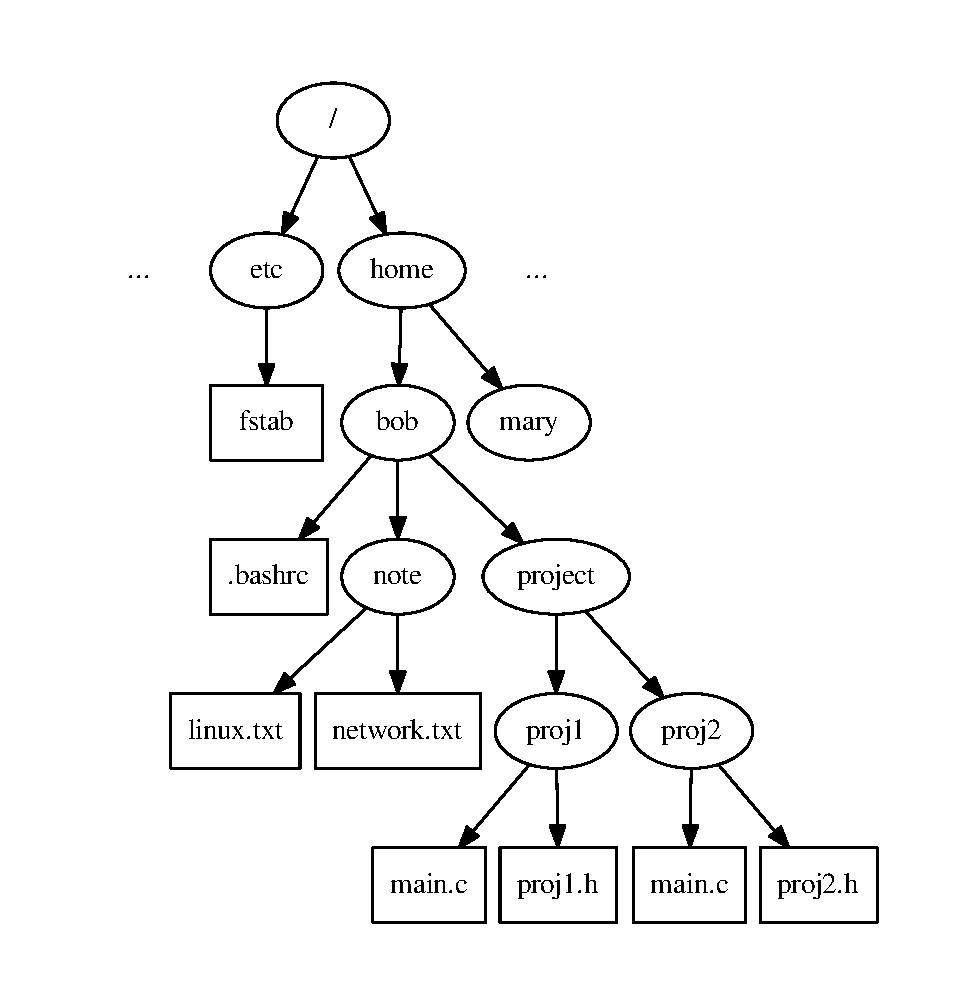
\includegraphics[width=.9\linewidth]{img/dirtree2.pdf}
\end{column}
\end{columns}
\end{frame}
\begin{frame}[fragile]
\frametitle{聊聊天吧}
\label{sec-4-2-17}
\begin{columns}
\begin{column}{0.5\textwidth}
\begin{block}{xiaobai}
\label{sec-4-2-17-1}


\begin{verbatim}
write laohei

hello, laohei!

I'm learning linux, it's fun!

Thank you!

Ctrl-d
 
\end{verbatim}
\end{block}
\end{column}
\begin{column}{0.5\textwidth}
\begin{exampleblock}{laohei}
\label{sec-4-2-17-2}


\begin{verbatim}

write xiaobai

hello, xiaobai.

Good luck.

You're welcome.

Ctrl-d
\end{verbatim}
\end{exampleblock}
\end{column}
\end{columns}
\end{frame}
\begin{frame}[fragile]
\frametitle{广而告之和请勿打扰}
\label{sec-4-2-18}
\begin{itemize}

\item wall\\
\label{sec-4-2-18-1}%
\begin{minted}[]{bash}
wall 'Pay attention! there comes BIG news!'
\end{minted}

\item mesg\\
\label{sec-4-2-18-2}%
\begin{minted}[]{bash}
mesg n      # 请勿打扰
mesg y      # 欢迎来访
\end{minted}

\item who\\
\label{sec-4-2-18-3}%
\begin{minted}[]{bash}
who -w      # 查看用户是否屏蔽消息
\end{minted}
\end{itemize} % ends low level
\end{frame}
\begin{frame}[fragile]
\frametitle{收发邮件}
\label{sec-4-2-19}
\begin{block}{xiaobai发邮件}
\label{sec-4-2-19-1}


\begin{verbatim}
mail laohei
help                 # 输入邮件主题
Hello, laohei, I have some problems with my linux.
Can you help me?     # 输入邮件正文
Ctrl-d               # 结束邮件内容并发送邮件
\end{verbatim}
\end{block}
\begin{exampleblock}{laohei收邮件和回复邮件}
\label{sec-4-2-19-2}


\begin{verbatim}
mail                  # 查看邮箱
p                     # 打印邮件
R                     # 回复邮件
Hello, xiaobai, I have time at 10:00 am on Friday.
.                     # 结束邮件内容
q                     # 退出
\end{verbatim}
\end{exampleblock}
\end{frame}
\begin{frame}[fragile]
\frametitle{关机/重启}
\label{sec-4-2-20}
\begin{itemize}

\item shutdown\\
\label{sec-4-2-20-1}%
\begin{minted}[]{bash}
shutdown -h now   #立即关机
shutdown +10 "System will shutdown in 10 minutes."
shutdown -c "Shutdown has been canceled."
\end{minted}

\item halt
\label{sec-4-2-20-2}%

\item poweroff
\label{sec-4-2-20-3}%

\item reboot
\label{sec-4-2-20-4}%
\end{itemize} % ends low level
\end{frame}
\subsection{4.3 命令行}
\label{sec-4-3}
\begin{frame}[fragile]
\frametitle{命令行格式}
\label{sec-4-3-1}
\begin{itemize}

\item 命令格式:命令 [选项]\ldots{} [参数]\ldots{}
\label{sec-4-3-1-1}%
\begin{itemize}

\item 选项(指示命令以什么方式执行)
\label{sec-4-3-1-1-1}%
\begin{itemize}

\item Unix简洁风:-a
\label{sec-4-3-1-1-1-1}%
\begin{itemize}

\item 多个选项可以共用一个减号
\label{sec-4-3-1-1-1-1-1}%
\end{itemize} % ends low level

\item GNU友好风:--all
\label{sec-4-3-1-1-1-2}%
\end{itemize} % ends low level

\item 参数(指示命令作用的对象,选项也可以有参数)
\label{sec-4-3-1-1-2}%

\item 注意
\label{sec-4-3-1-1-3}%
\begin{itemize}

\item 命令、选项和参数之间要有空格(选项及其参数之间有时可以没有空格)
\label{sec-4-3-1-1-3-1}%

\item 选项及其参数之间不能放置其他选项
\label{sec-4-3-1-1-3-2}%
\end{itemize} % ends low level
\begin{exampleblock}{命令行示例}
\label{sec-4-3-1-1-3-3}


\begin{minted}[]{bash}
tar -cvf boot.tar /boot #选项f必须放在最后!
\end{minted}
\end{exampleblock}
\end{itemize} % ends low level
\end{itemize} % ends low level
\end{frame}
\begin{frame}[fragile]
\frametitle{命令类型}
\label{sec-4-3-2}
\begin{itemize}

\item 外部命令:具有独立的可执行文件\\
\label{sec-4-3-2-1}%
\begin{minted}[]{bash}
which cat           #查看cat可执行文件路径
type cat            #查看命令类型
\end{minted}

\item 内部命令:shell内置命令,没有独立可执行文件\\
\label{sec-4-3-2-2}%
\begin{minted}[]{bash}
which exit          #找不到,因为exit是内部命令
type exit
\end{minted}

\item 命令别名:为命令所取的别名\\
\label{sec-4-3-2-3}%
\begin{minted}[]{bash}
which ls            #是同名外部命令ls的别名
type ls
alias               #查看所有别名
alias see 'cat -n'  #定义别名
unalias see         #删除别名
\end{minted}
\end{itemize} % ends low level
\end{frame}
\begin{frame}
\frametitle{命令搜索顺序}
\label{sec-4-3-3}
\begin{itemize}

\item shell如何找到我们要执行的命令?
\label{sec-4-3-3-1}%
\begin{enumerate}
\item 是否是别名?
\item 是否是内部命令?
\item 是否是外部命令?
\begin{itemize}
\item 从左到右依次搜索PATH环境变量包含的路径
\item 一旦在某条路径中找到所要执行的命令,则不再搜索后续路径
\end{itemize}
\item 找到了则执行命令;找不到则给出提示(一定要仔细看提示!)。
\end{enumerate}
\end{itemize} % ends low level
\end{frame}
\begin{frame}
\frametitle{选项a-n巡礼}
\label{sec-4-3-4}


\begin{center}
\begin{tabular}{1\textwidth}{ll}
 选项  &  含义                                    \\
\hline
 -a    &  all, append                             \\
 -b    &  buffer, block, batch                    \\
 -c    &  command, check                          \\
 -d    &  debug, delete, directory                \\
 -D    &  define                                  \\
 -e    &  excute, edit, exclude, expression       \\
 -f    &  file, force                             \\
 -h    &  header, help                            \\
 -i    &  initialize, interactive                 \\
 -I    &  include                                 \\
 -k    &  keep, kill                              \\
 -l    &  list, long, load, login                 \\
 -m    &  message, mail, mode, modification-time  \\
 -n    &  number, not                             \\
\end{tabular}
\end{center}
\end{frame}
\begin{frame}
\frametitle{选项o-z巡礼}
\label{sec-4-3-5}


\begin{center}
\begin{tabular}{ll}
 选项    &  含义                   \\
\hline
 -o      &  output                 \\
 -p      &  port, protocol         \\
 -q      &  quite                  \\
 -r(-R)  &  recurse, reverse       \\
 -s      &  silent, subject, size  \\
 -t      &  tag                    \\
 -u      &  user                   \\
 -v      &  verbose, version       \\
 -V      &  version                \\
 -w      &  width, warning         \\
 -x      &  debug, extract         \\
 -y      &  yes                    \\
 -z      &  zip                    \\
\end{tabular}
\end{center}
\end{frame}
\begin{frame}
\frametitle{命令行编辑}
\label{sec-4-3-6}
\begin{itemize}

\item 命令自动完成:Tab键
\label{sec-4-3-6-1}%

\item 快捷键\\
\label{sec-4-3-6-2}%
\begin{center}
\begin{tabular}{ll}
 按键    &  功能               \\
\hline
 Ctrl-a  &  移动光标至行首     \\
 Ctrl-e  &  移动光标至行尾     \\
 Ctrl-d  &  向后删除/结束输入  \\
 Ctrl-h  &  向前删除           \\
 Ctrl-k  &  向后删除到行尾     \\
 Ctrl-u  &  向前删除到行首     \\
 Ctrl-c  &  中止执行           \\
 Ctrl-p  &  上一条命令         \\
 Ctrl-n  &  下一条命令         \\
\end{tabular}
\end{center}


\end{itemize} % ends low level
\end{frame}
\begin{frame}[fragile]
\frametitle{命令历史}
\label{sec-4-3-7}
\begin{itemize}

\item 命令历史: 可用上下箭头翻阅用过的命令
\label{sec-4-3-7-1}%
\begin{itemize}

\item 命令历史保存在内存中,用户注销时保存至.bash$_{\mathrm{history}}$文件,用户登录时从该文件加载至内存。
\label{sec-4-3-7-1-1}%

\item 命令历史长度由环境变量HISTSIZE的值决定\\
\label{sec-4-3-7-1-2}%
\begin{minted}[]{bash}
echo $HISTSIZE  #打印环境变量HISTSIZE的值
history         #列出所有历史命令
!20             #执行第20条命令
!!              #执行上一条命令
!-1             #同上
!ls             #执行最近一条以ls开头的命令
Ctrl-r
doc             #搜索最近一条包含doc的命令
                #按回车执行,按左右键编辑
history -c      #清除命令历史
\end{minted}
\end{itemize} % ends low level
\end{itemize} % ends low level
\end{frame}
\begin{frame}
\frametitle{屏幕控制}
\label{sec-4-3-8}
\begin{itemize}

\item 向上翻页屏幕输出:Shift-PgUp
\label{sec-4-3-8-1}%

\item 向下翻页屏幕输出:Shift-PgDn
\label{sec-4-3-8-2}%

\item 暂停屏幕输出:Ctrl-s
\label{sec-4-3-8-3}%

\item 恢复屏幕输出:Ctrl-q
\label{sec-4-3-8-4}%

\item 清屏:clear(快捷键为Ctrl-l)
\label{sec-4-3-8-5}%

\item 重置终端:reset
\label{sec-4-3-8-6}%
\end{itemize} % ends low level
\end{frame}
\subsection{4.4 获取帮助}
\label{sec-4-4}
\begin{frame}[fragile]
\frametitle{man (manual)}
\label{sec-4-4-1}


\begin{minted}[]{bash}
man ls         #查看ls的手册页
               # h(获取帮助)
               # q(退出)
man man        #查看man手册的手册页
man passwd
man 5 passwd   #查看第5章的passwd手册页
whatis cp      #查看命令简要描述,等同于man -f cp
apropos who    #根据关键字查询,等同于man -k who
\end{minted}
\end{frame}
\begin{frame}[fragile]
\frametitle{help}
\label{sec-4-4-2}


\begin{minted}[]{bash}
help        #列出所有内部命令
help cd     #显示内部命令cd的帮助
cat --help  #显示外部命令cat的简明帮助
\end{minted}
\end{frame}
\begin{frame}[fragile]
\frametitle{info  多级结构,且支持超链接}
\label{sec-4-4-3}


\begin{minted}[]{bash}
info        #打开info首页
info who    #打开who的info页
            #h(获取帮助)H(入门指南)
            #q(退出)
\end{minted}
\end{frame}
\begin{frame}
\frametitle{其他帮助}
\label{sec-4-4-4}
\begin{itemize}

\item 软件包自带文档: /usr/share/doc
\label{sec-4-4-4-1}%

\item 软件官方网站提供的文档
\label{sec-4-4-4-2}%

\item Internet: 搜索引擎、网站博客、技术论坛
\label{sec-4-4-4-3}%

\item book: 图书馆、电子书
\label{sec-4-4-4-4}%
\end{itemize} % ends low level
\begin{block}{提问原则}
\label{sec-4-4-4-5}

\begin{enumerate}
\item 在经过自己的思考和实践后再请教别人!
\item 请把问题描述清楚!
\end{enumerate}
\end{block}
\end{frame}
\begin{frame}
\frametitle{学习QQ群}
\label{sec-4-4-5}
\begin{columns}
\begin{column}{0.5\textwidth}
%% 加群
\label{sec-4-4-5-1}

\begin{itemize}
\item 群号:494598324
\item 实名验证:班级+姓名
\end{itemize}
\end{column}
\begin{column}{0.5\textwidth}
%% 二维码
\label{sec-4-4-5-2}


\includegraphics[width=.9\linewidth]{img/learning-linux.png}
\end{column}
\end{columns}
\end{frame}

\end{document}
